%\documentclass[a4paper,20pt]{report}
\documentclass[a4paper,18.pt]{article}
\makeindex
\usepackage{booktabs}
\usepackage{epsfig}
\usepackage{graphicx}
\usepackage{epstopdf}
\usepackage{amsmath}
\usepackage{rotating}
\usepackage{caption}
\usepackage{subfig}

% Title Page
%\textwidth 15 true cm
%\textheight 25 true cm
%\headheight  14pt
%\headsep    16pt
%\footskip   27pt
%\marginparsep 10pt
%\marginparwidth  100pt
% \def\marginset#1#2{
% \setlength{\oddsidemargin}{#1}
% \iffalse
% \reversemarginpar
% \addtolength{\oddsidemargin}{\marginparsep}
% \addtolength{\oddsidemargin}{\marginparwidth}
% \fi
% 
%   \setlength{\evensidemargin}{0mm}
% \iffalse
% \addtolength{\evensidemargin}{\marginparsep}
% \addtolength{\evensidemargin}{\marginparwidth}
% \fi
% 
%   % \paperwidth = h + \oddsidemargin+\textwidth+\evensidemargin + h
% \setlength{\hoffset}{\paperwidth}
% \addtolength{\hoffset}{-\oddsidemargin}
% \addtolength{\hoffset}{-\textwidth}
% \addtolength{\hoffset}{-\evensidemargin}
% \setlength{\hoffset}{0.5\hoffset}
% \addtolength{\hoffset}{-1in}           % h = \hoffset + 1in
% 
%   \setlength{\voffset}{-1in}             % 0 = \voffset + 1in
% \setlength{\topmargin}{\paperheight}
% \addtolength{\topmargin}{-\headheight}
% \addtolength{\topmargin}{-\headsep}
% \addtolength{\topmargin}{-\textheight}
% \addtolength{\topmargin}{-\footskip}
% \addtolength{\topmargin}{#2}
% \setlength{\topmargin}{0.5\topmargin}
% }
% 
% \marginset{11mm}{11mm}
\title{E08014 Cross Section Extraction}
%\subtitle{A note of $x>2$ cross section extraction package}
\author{Zhihong Ye\\ University of Virginia}

\begin{document}
\maketitle

\section{Instruction}

The formula of cross section as a function of $x_{bj}$ is written as following:
\begin{equation}
 \frac{d\sigma}{d\Omega dE'}(x_{bj}^{i}) = \frac{N_{EX}^{i} \epsilon_{pion\_rej}}{N_{tg} N_{e} \epsilon_{det} \epsilon_{track}} \frac{N_{MC}^{gen}}{N_{MC}^{i} \Delta\Omega_{MC} \Delta E'_{MC}},
\label{xs_eq}
\end{equation}
where each quantities will be discussed individually in the following sections.

A package of inclusive electrons scattering cross section extraction has been developed for E08-014 experiment data. The basic structure of the code and files can be viewed from the chart bellow.

\begin{figure}[h!]
 \centerline{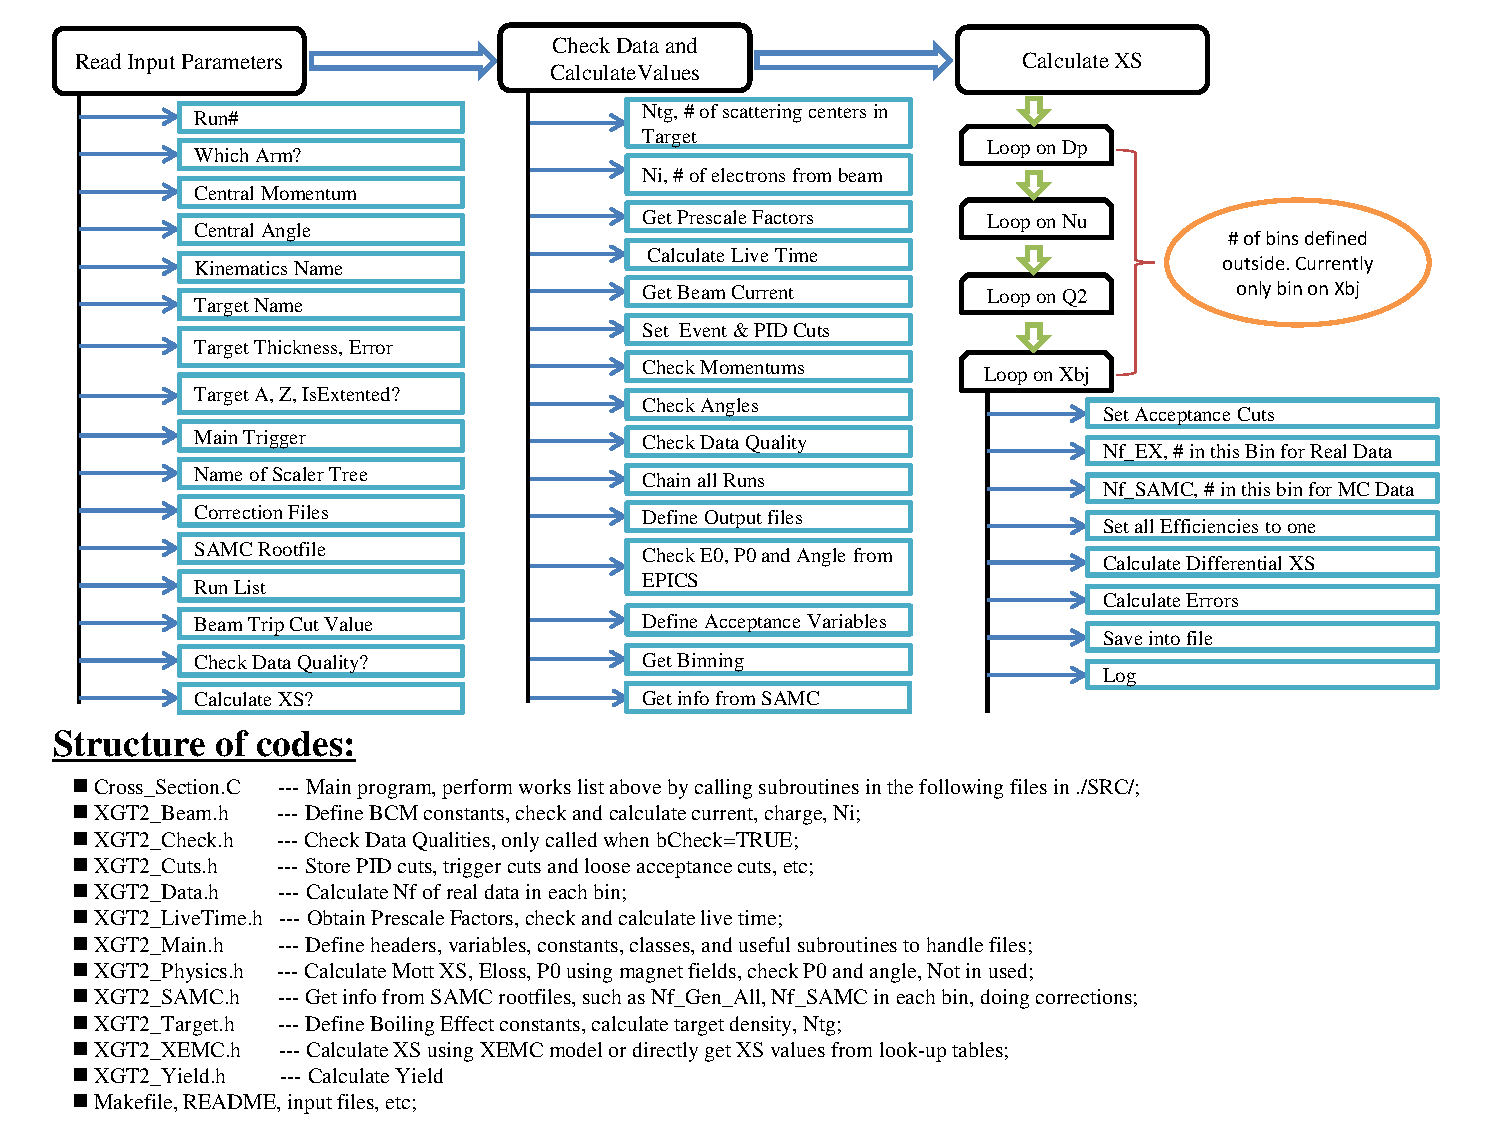
\includegraphics[width=0.95\linewidth]{../figures/XS_Chart.eps}}
 \caption[Basic structure of XS package]{Basic structure of the cross section extraction package}
 \label{xs_chart}
\end{figure}

\section{Step by Step}

\subsection{Beam Charge}

Base on the work of BCM calibration by Patricia, we are able to calculate total electron charge or the total number of electrons delivered from beam in one run. However, if we remove events taken during beam trip, the amount of electron charge accumulated when beam currents were lower than requesting values will need to be subtracted. A script was written to calculate charge and current between two consecutive scaler events, for example, the charge and current calculated base on beam charge monitor (BCM) $U_{1}$ for $ith$ scaler event are given by:
\begin{equation}
  \Delta C_{i}^{U_{1}} = C_{i+1}^{U_{1}} - C_{i}^{U_{1}},  I_{i}^{U_{1}} = \Delta C_{i}^{U_{1}}/(T_{i+1}-T_{i}),
\end{equation}
where $\Delta C_{i+1}^{U_{1}}$ gives the calibrated values of charge accumulated between two consecutive scaler events happening at CPU clock $T_{i+1}$ and $T_{i}$, of which the difference is normally set to be three seconds. Values of charge and current for BCM $U_{1}, U_{3}, D_{1}$ and $D_{3}$ are calculated similarly and their average value, $C_{i}^{avg}$ and $I_{i}^{avg}$, are assigned to all events happening during this time window. Then a beam trip cut will remove events with currents lower than the cut value, and the total number of electrons from the beam for each run is re-evaluated:
\begin{equation}
  N_{e} = \sum_{i^{*}} \Delta C_{i^{*}}^{avg}(I_{i^{*}}^{avg}>I_{beam\_trip\_cut}),
\end{equation}
where $i^{*}$ means summarizing scaler events with beam current $I_{i^{*}}$ higher than the cutting value $I_{beam\_trip\_cut}$, which we chose to be half of the value we requested during the experiment.

During the experiment, Left BCM scalers did not work properly so we used the values of charge calculated from HRS-R BCM for HRS-L data since two arm shared the same DAQ system. 

\subsection{Targets}
\subsubsection{Boiling Effect}
Total number of scattering centers (or nuclei) in a target with known thickness is given by:
\begin{equation}
 N_{tg} = \frac{\rho\cdot l \cdot N_{a}}{A},
\end{equation}
where $\rho$ is the target density in $g/cm^{3}$, $l$ is the target length in cm, $N_{a}$ is the Avogadro's number and A is the nuclear number of the target. 

For cryogenic long targets, $^{2}H, ^{3}He$ and $^{4}He$ used in this experiment, $l$ should be equal to the length of targets after we cut on vertex variables, instead of the design length. Heat deposits in the target system when beam is on and cause the variation of target densities. This so called boiling effect are needed to be corrected:
\begin{equation}
  \rho_{cor} = \rho \cdot (1.0 - B \cdot I /100),
\end{equation}
where $I$ and $B$ are the value of beam current and the boiling factor for a specific target, respectively. Study of boiling effect is performed by Patrica Solvignon %\ref{boiling_patricia}. 

\subsubsection{Density Non-Linearity}

\begin{figure}[ht]
 \begin{center}
  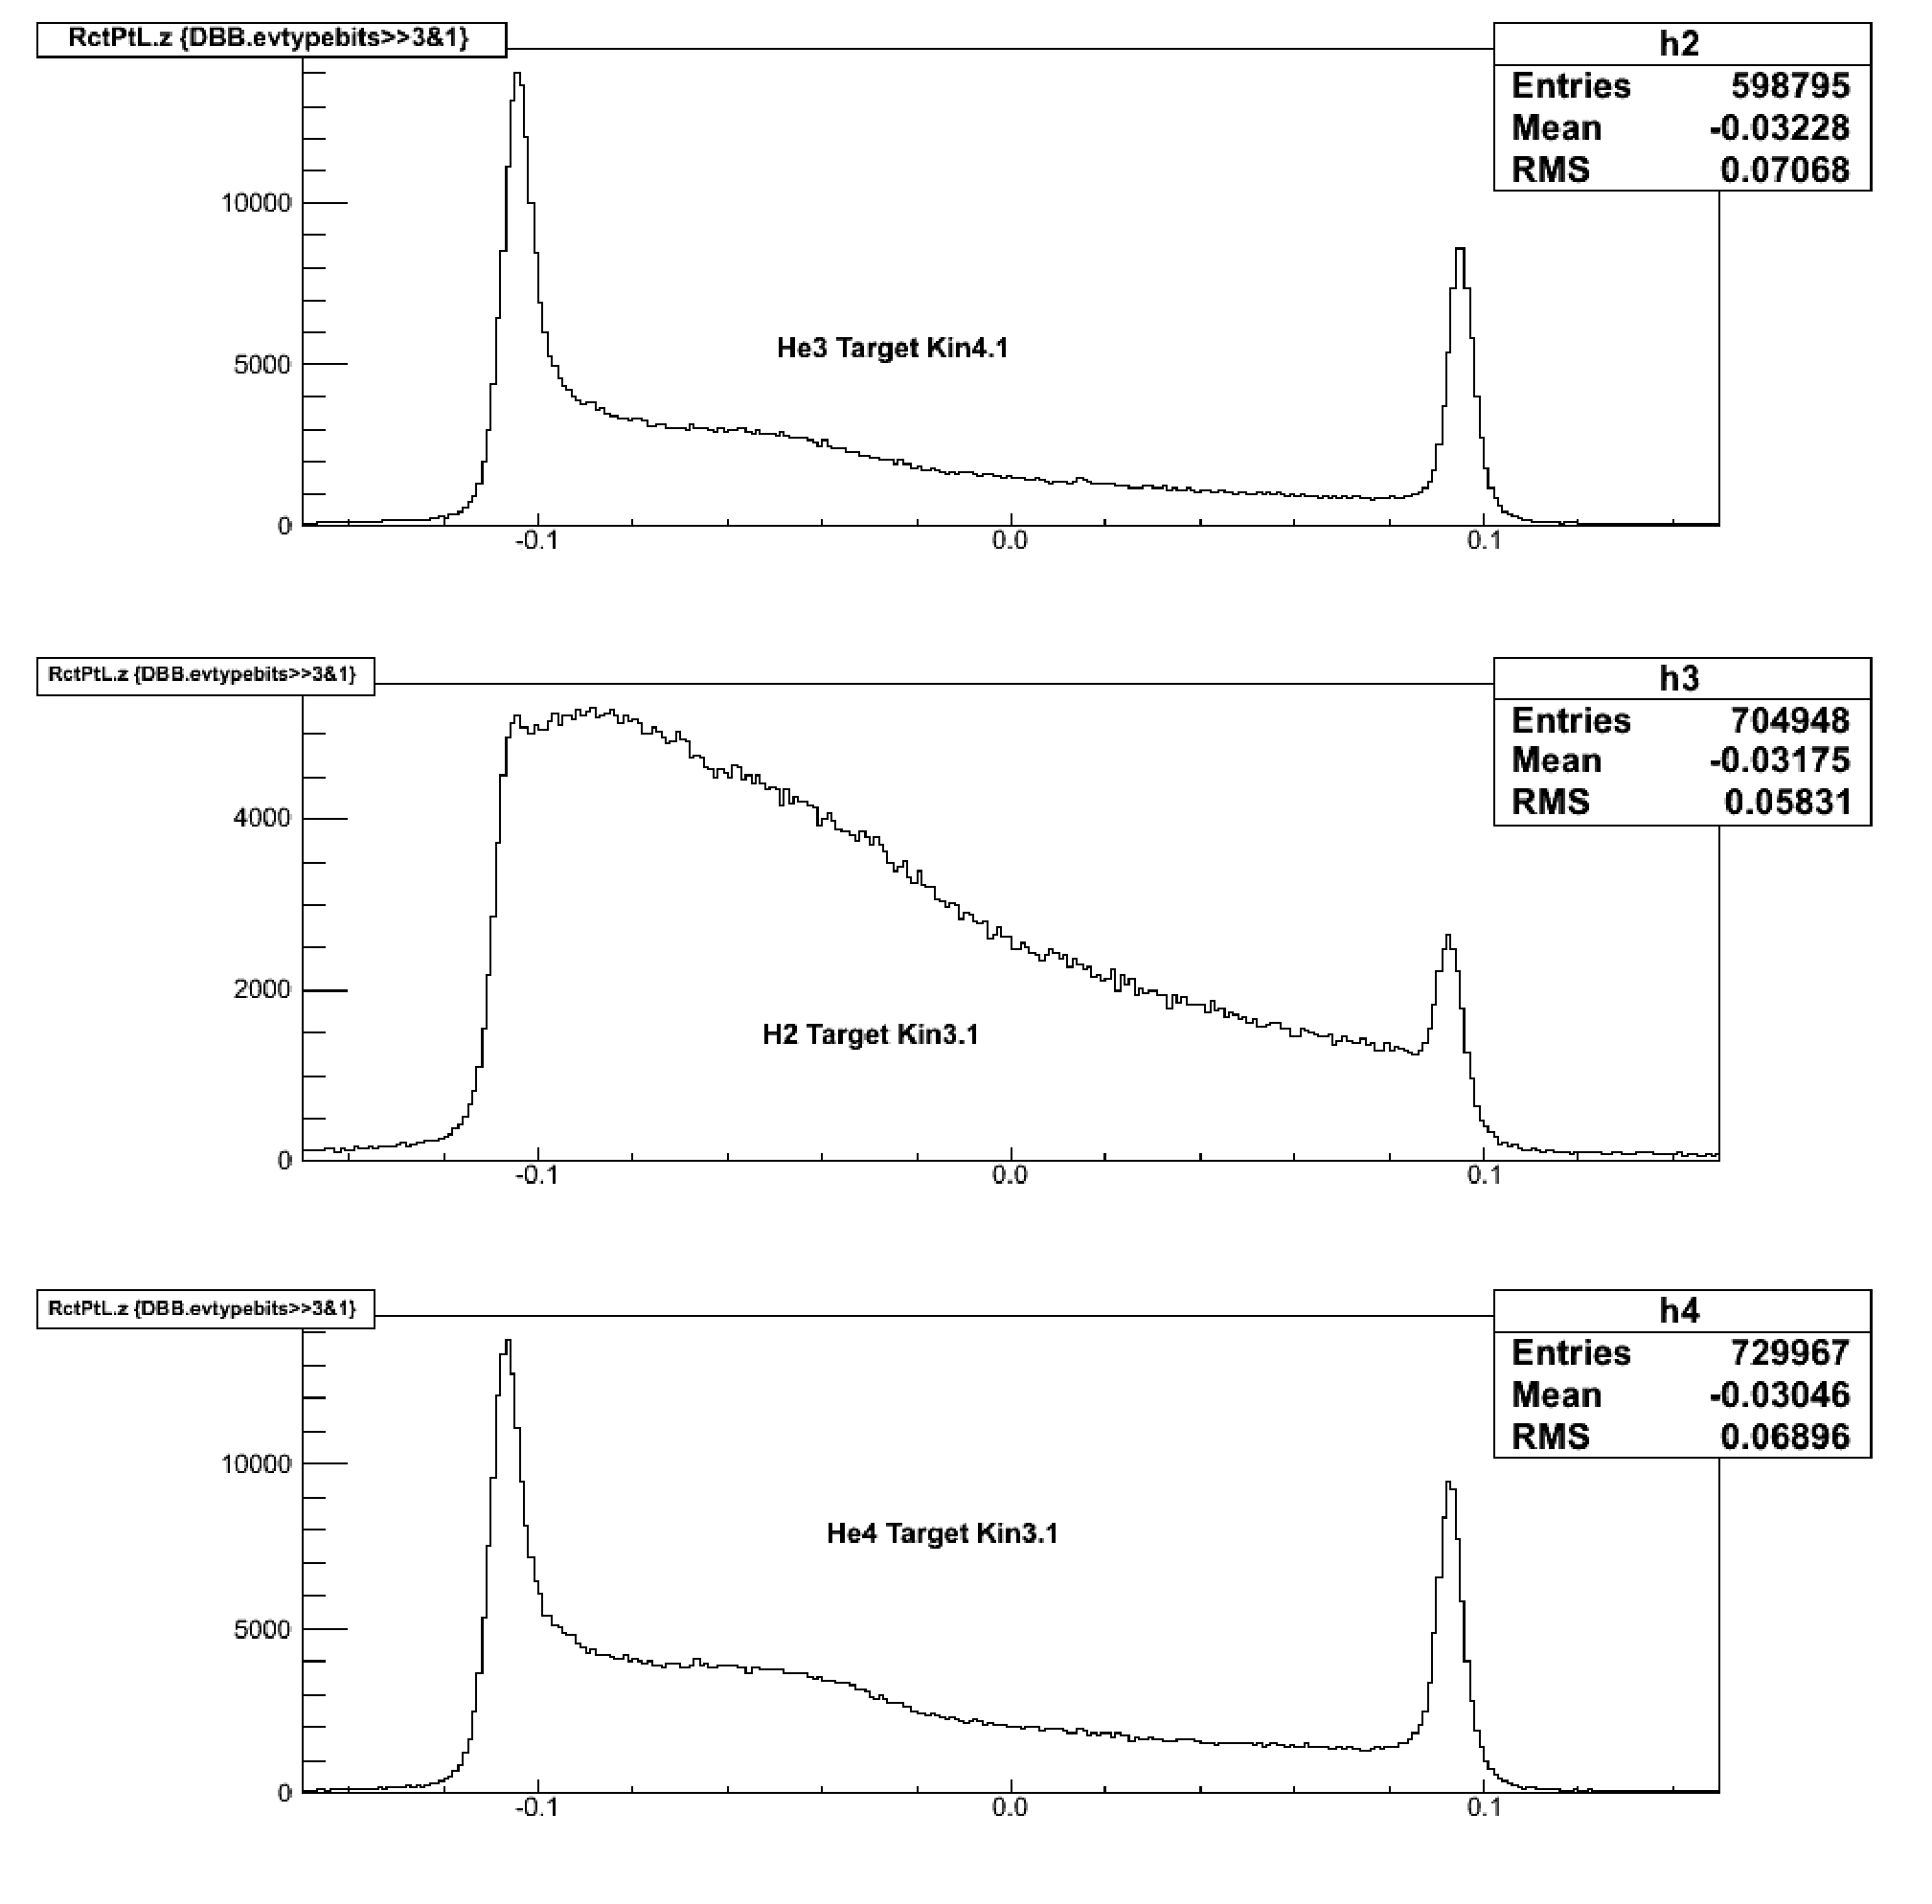
\includegraphics[width=0.6\textwidth]{../figures/target/L_Cryo_RPZ.eps}
  \caption[Long target bumps due to non-uniform density distribution]{Long target bumps due to non-uniform density distribution}
  \label{he3_bump}
 \end{center}
\end{figure}

During E08-014 experiment, we were using $20cm$ $^{2}H, ^{3}He$ and $^{4}He$ long cryogenic targets. The design of cooling system caused targets had higher density upstream and lower density downstream, even without beam applied on targets. The boundary of this two regions were near around $2cm$ toward upstream end-cup with an range of $4cm$ transition region, where a bump clearly appears when plotting vertex distribution of one of those targets (Fig.\ref{he3_bump}). If we plot the distribution at different beam currents, we will see how the bumps become significant when beam increasing (Fig.\ref{bump_current}).

\begin{figure}[ht!]
 \begin{center}
 \subfloat[$^{2}H$]{
  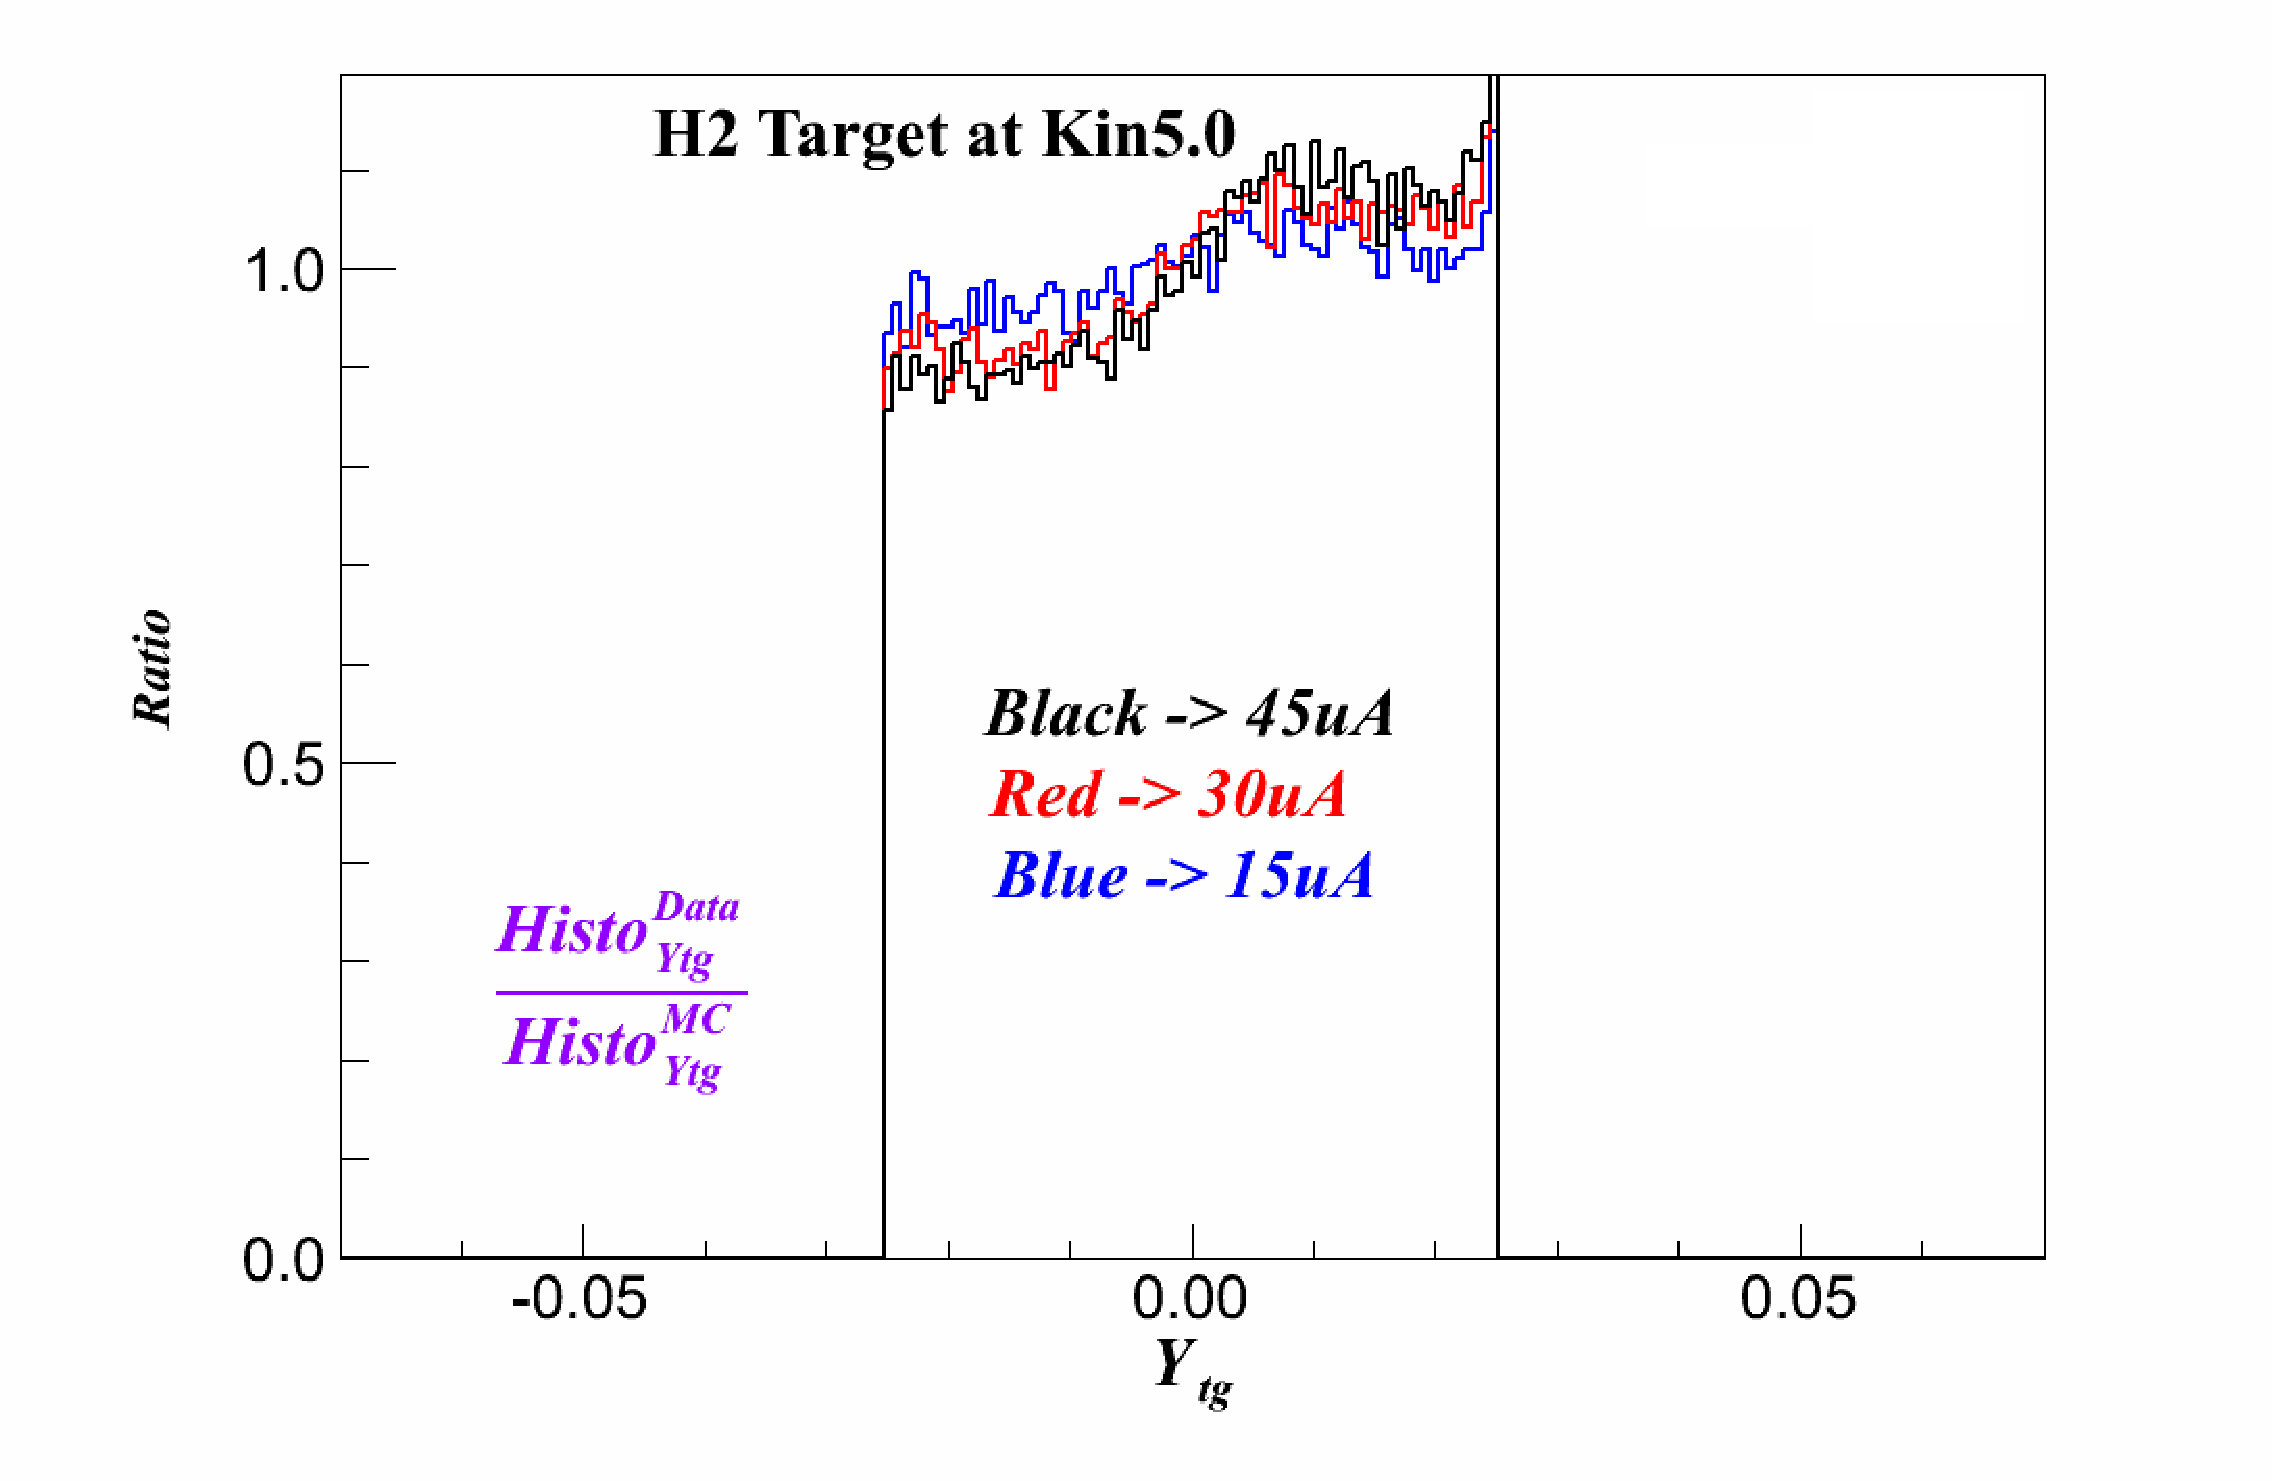
\includegraphics[width=0.6\textwidth]{../figures/target/H2_Histo_Ratio.eps}
 } 
\\
 \subfloat[$^{3}He$]{
  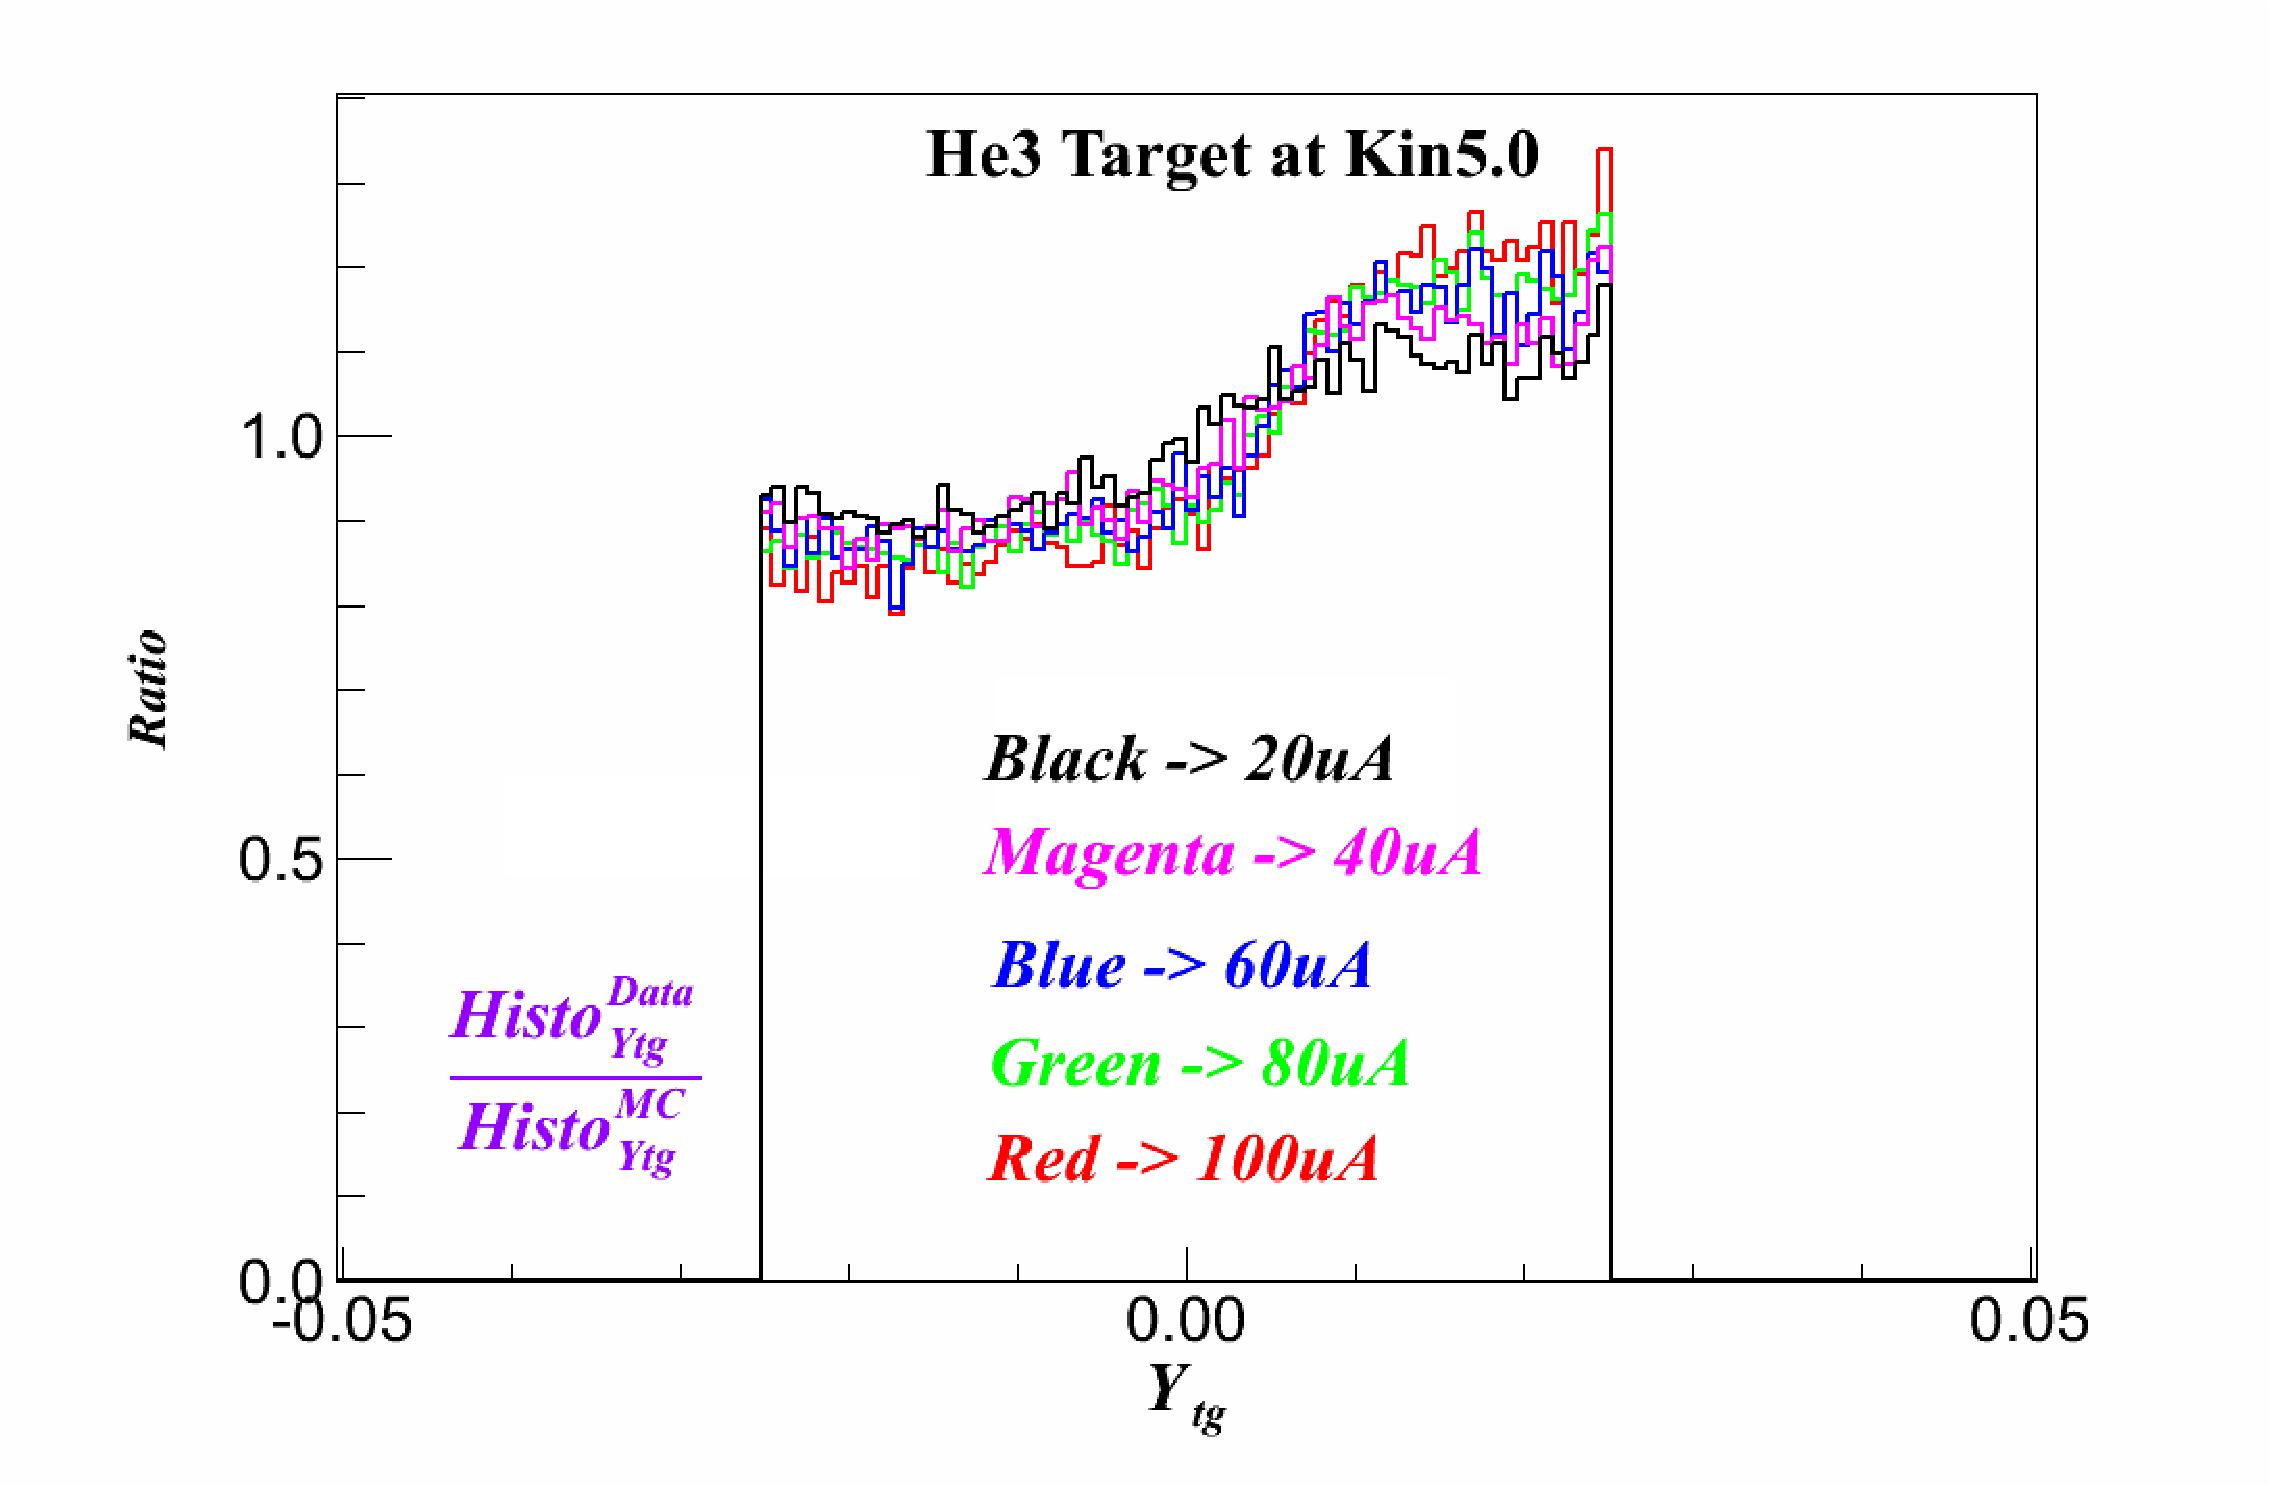
\includegraphics[width=0.6\textwidth]{../figures/target/He3_Histo_Ratio.eps}
}
\\
\subfloat[$^{4}He$]{
  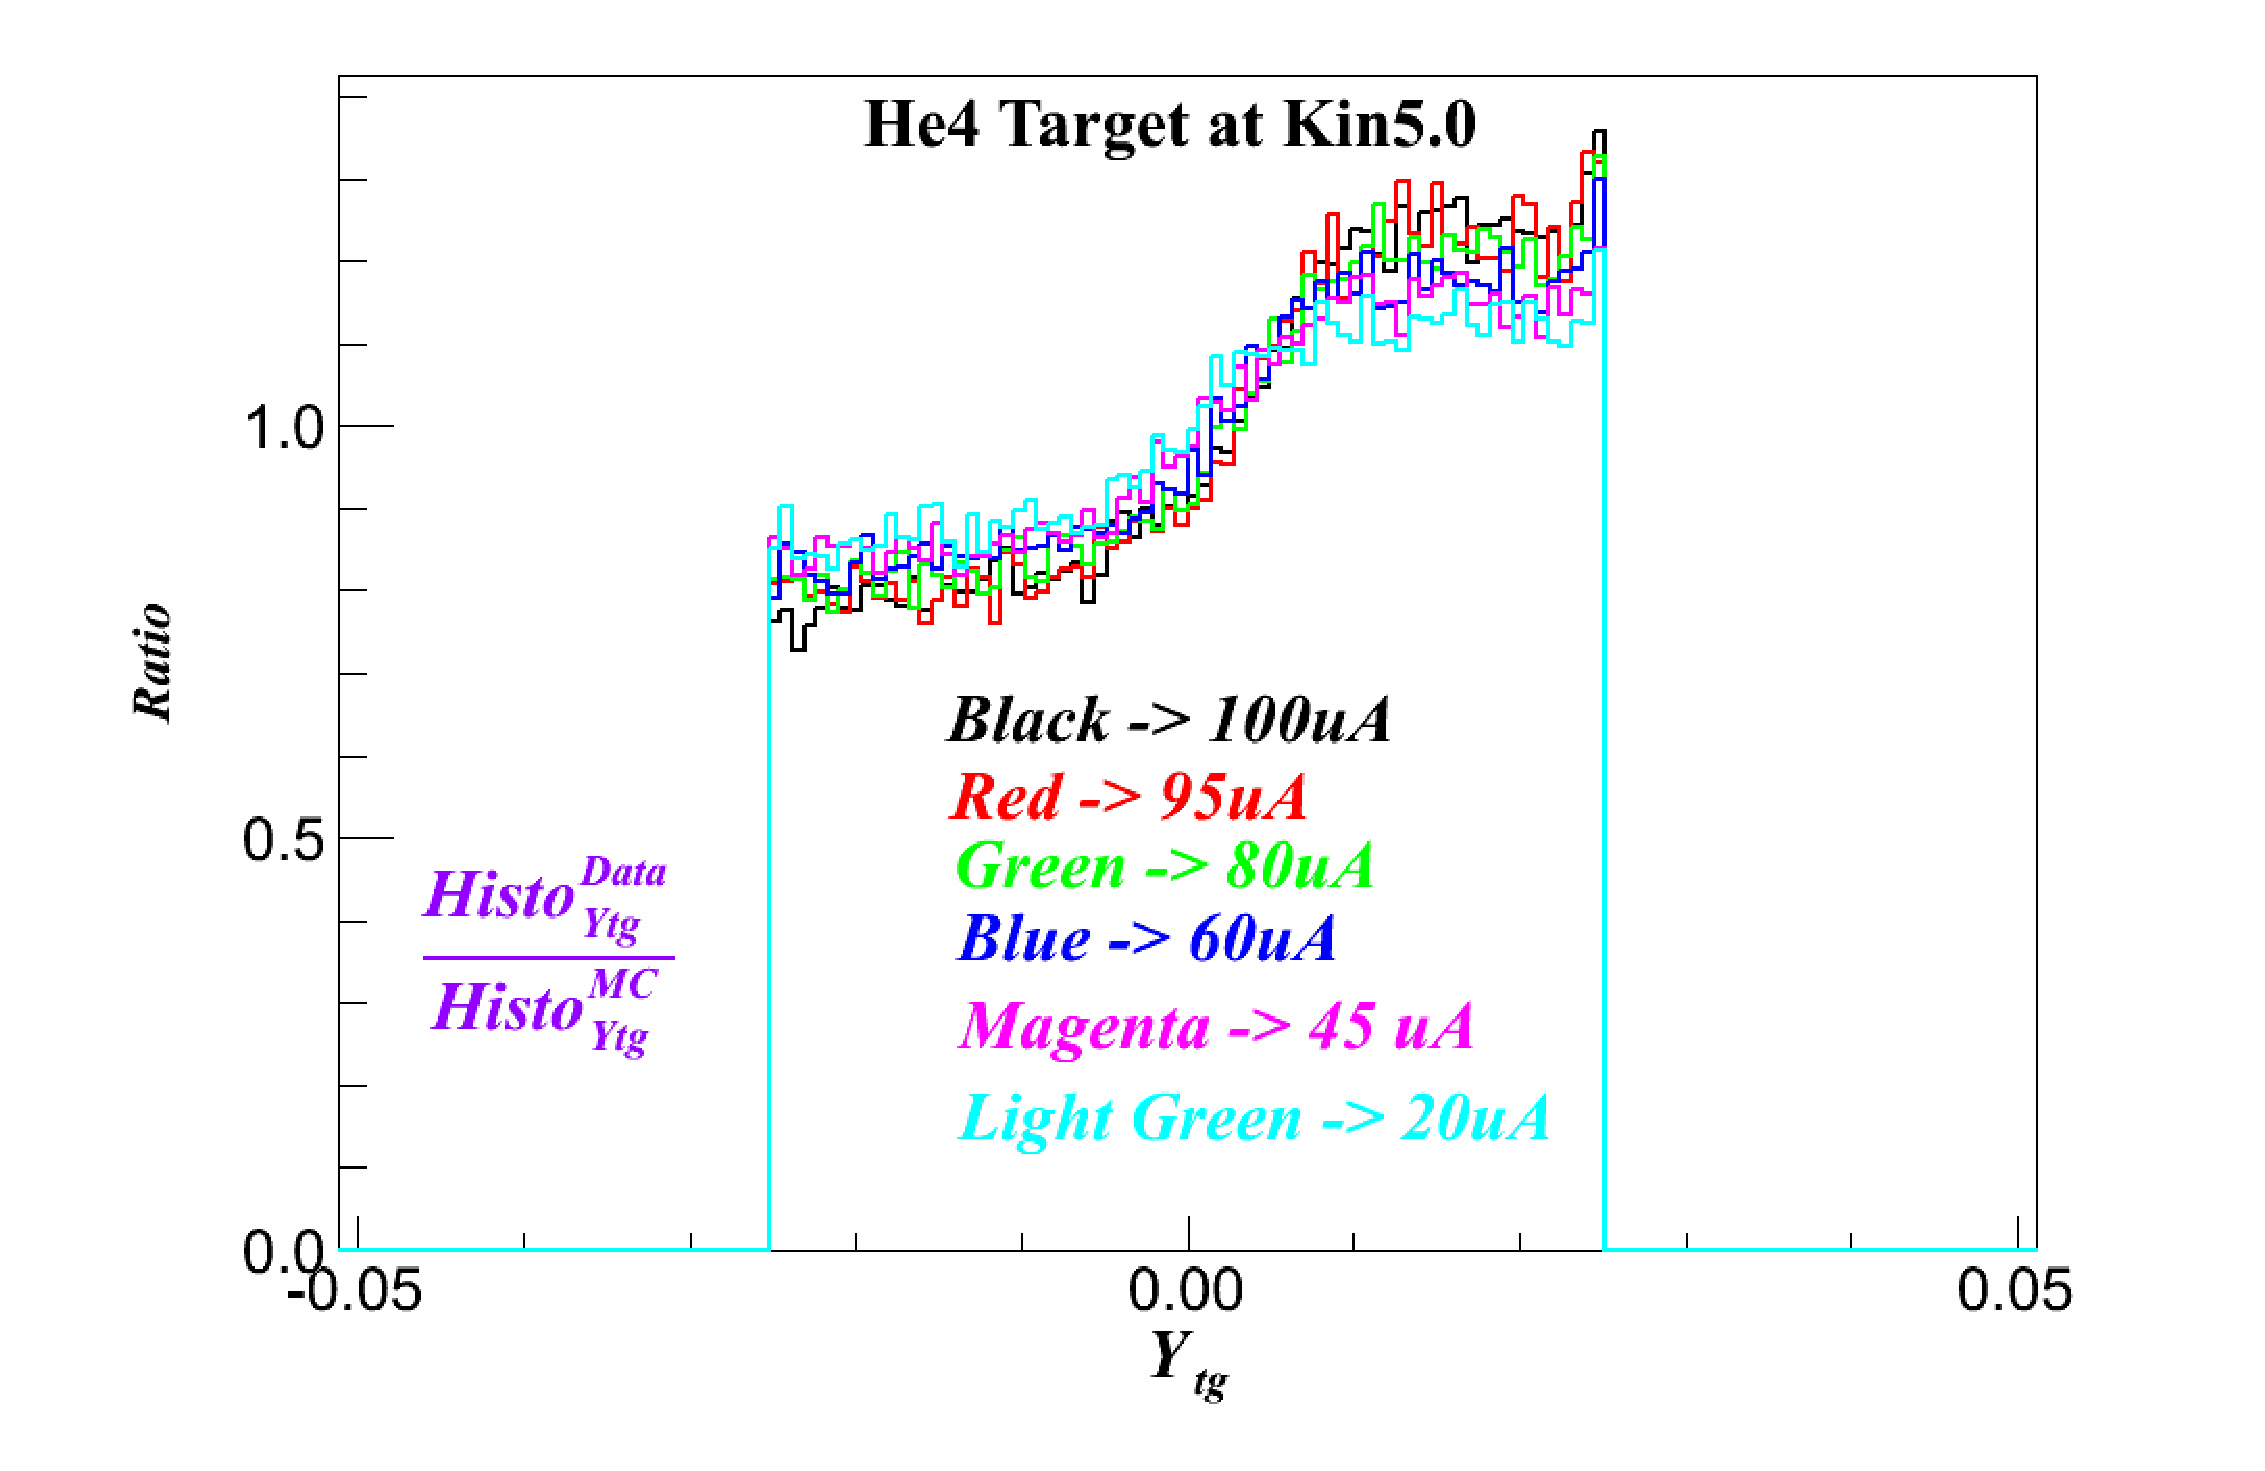
\includegraphics[width=0.6\textwidth]{../figures/target/He4_Histo_Ratio.eps}
}
 \caption[Long target bumps changing with beam current]{Long target bumps changing with beam current}
 \label{bump_current}
\end{center}
\end{figure}

The density non-uniformity of long targets causes a series of problems when extracting cross section results. First of all, total number of nuclei in the while long target cell for each target is needed to be carefully calculated, since the estimated densities using feedback information of temperature and pressure can not directly give the correct answer. Instead, absolute density values in each part of one target have to be known, which are heavily relied on the design of the target system. Secondly, due to the fact that more events come from the upstream part of one target where there are more scattering centers, hence a false physics phenomenal is introduced into the cross sections. Since we don't bin on $Y_{tg}$, this effect has to be corrected before we calculate cross sections. Last but not least, radiation correction will be much more complicate than one assuming the uniform target density. Loss of initial and final energy of scattered electrons would be harder to estimate, and the parameters for radiation correction, such as total radiation length, is required to be calculated differently at different reaction points. A much more detail discussion of solving this problem using cross section models and Monte Carlo simulation is given latter in this section.

\subsection{Live Time}

DAQ running at high trigger rates generally decreases live time, or in other words,increases dead time. Dead time is mainly composed of hardware dead time and electronic dead time. Hardware dead time comes from the fact that detectors can not identify two or more particles coming nearly at the same time. Electronic dead time, which is the major source, arises when electronic modules, including computer system, skip the next event when they are still processing the current event, and cause those events not recorded by DAQ system. To reduce dead time we assign a prescale factor to each trigger type to control the total trigger rates. The values of pre-scale factors are stored in each run and can be read out to calculate the actually total number of events for different types. 

We can evaluate the electronic dead time by using the fact that events not recorded by DAQ are still counted by scalers. For each trigger type in each run, the value of live time is given by the ratio of total number of events recorded by DAQ before prescaling and the total counts in scalers:
\begin{equation}
  LiveTime_{T_{i}} = \frac{N_{T_{i}}^{DAQ} PS_{T_{i}}}{N_{T_{i}}^{Scaler}},
\end{equation}
where $N_{T_{i}}^{DAQ}$ and $N_{T_{i}}^{Scaler}$ are total number of DAQ events and scaler counts in one run after removing events taking during beam trip.

\subsection{Efficiencies}

Detectors do not work in 100\% performance and the inefficiencies of detectors caused by hardware and software are needed to be evaluated and corrected when extracting cross sections. The analysis results show that for E08014 data, the detection efficiencies of all detectors are very close to $99\%$ and meanwhile, loose PID cuts are good enough to eliminate most of pions and their cut efficiencies are also close to 99\%. So during the cross section calculation, we don't apply corrections of those efficiencies but only quote $1\%$ of the systematic errors.


\subsubsection{Triggers}

 There are mainly three aspects that determine the trigger efficiency~\cite{R_Bock}, first one of which is the trigger algorithm designed to compromise between highly reducing background and keeping most of good events, second one of which would be the dead time caused by electronics and performance of detectors involved in the trigger system, and the last one of which is the writing speed of computer systems. It is important to avoid double counting detectors' inefficiencies when evaluating trigger efficiencies. The definition of trigger efficiency generally includes the inefficiency of scintillator counters and the formula is written as:
\begin{equation}
 \epsilon_{trigger\_eff} = \frac{PS1(3)\times N_{T1(3)}}{PS1(3) \times N_{T1(3)}+PS2(4)\times N_{T2(4)}},
 \label{trigger_eff}
\end{equation}
where $N_{T1(2,3,4)}$ is number of events triggered by T1(2,3,4) after prescaled by PS1(2,3,4). Traditionally in Hall-A T1(3) is designed by requesting coincidence trigger signals between S1 and S2m, while T2(4) includes signals from GC in the trigger, which should carry the inefficiency effect of GC. However, during the E08014 experiment, T1(3) was modified to include GC signals in trigger, so the detection inefficiency of GC is canceled from the equation. Fig.\ref{trig_eff} shows that the trigger efficiencies of our data on both arm were better than 99\%.

%\clearpage
%\begin{figure}[h!]
 \begin{center}
\parbox[t]{0.8\textwidth}{
\centerline{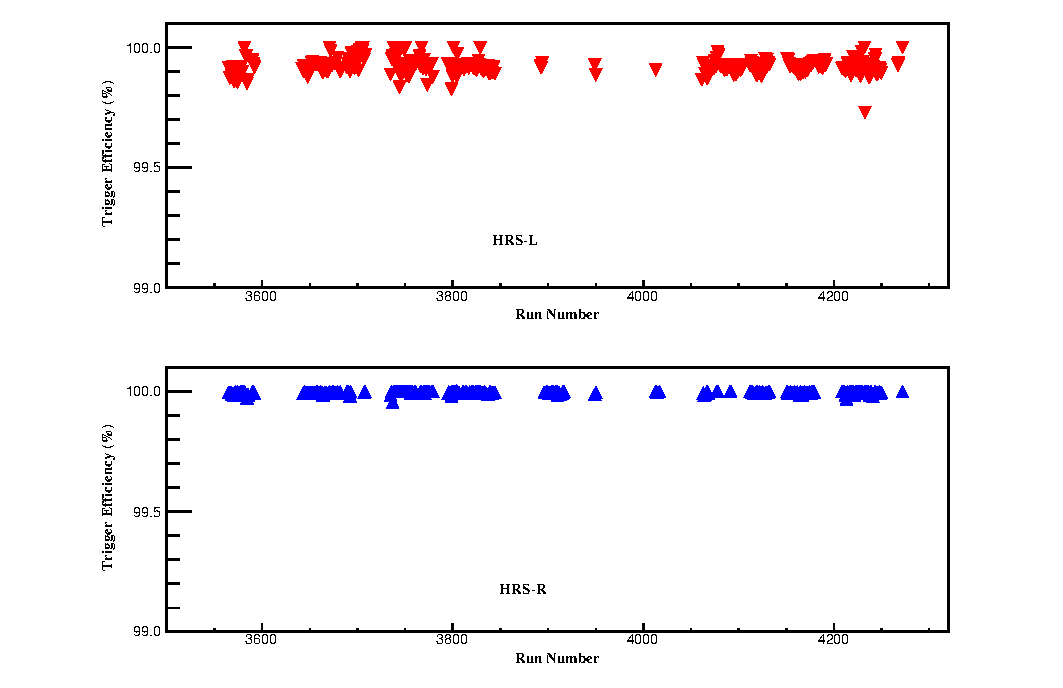
\includegraphics[width=1.\linewidth]{../figures/scin/Trigger_Eff.eps}}
\captionof{figure}{\footnotesize{Trigger Efficiencies}}
\label{trig_eff}
}
%\end{figure}
\\
%\begin{figure}[h!]
\parbox[t]{0.8\textwidth}{
\centerline{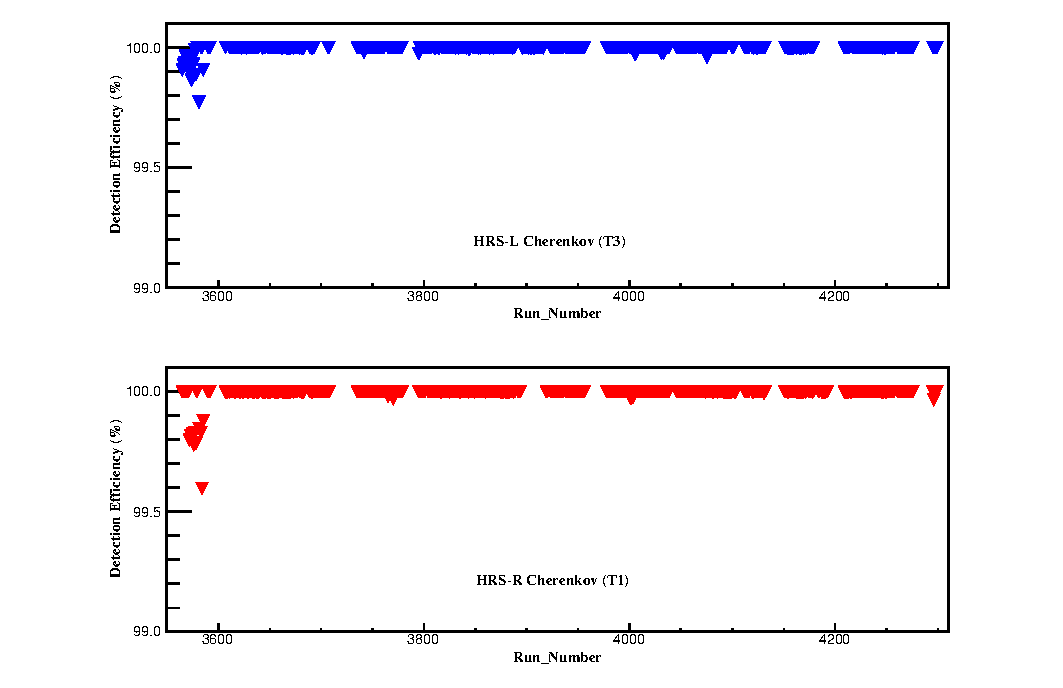
\includegraphics[width=1.\linewidth]{../figures/cer/Cer_Det_Eff.eps}}
\captionof{figure}{\footnotesize{Gas Cherenkov Detection Efficiency}}
\label{cer_det_eff}
}
 \end{center}
%\end{figure}


\subsubsection{VDCs}

Inefficiency of VDCs caused by hardware is negligible and the major source is from the mis-reconstruction of particle tracks during the tracking algorithm. Only one-track events are kept for analysis, and the good events threw away by zero-track and multi-tracks cut are corrected by the one-track efficiency defined as:
\begin{equation}
 \epsilon_{one\_track\_eff} = \frac{N_{Track=1}}{N_{0<=Tracks<=4}}
\end{equation}
 It is very important to select correct electron samples when calculating values of one-track efficiency. We need to avoid applying cuts on variables that require tracking information, such as variables at focal plane and target plane, and cutting on other VDC variables will introduce other sources of inefficiencies. Cluster-reconstructed variables of calorimeters, such as E/P, can not be used when cutting electrons. cosmic ray events should also be removed since they come with big angles. We could not cut on TOF $\beta$ to suppress cosmic ray background due to the TDC multi-peaks issues on some scintillator bars. During the analysis, we used quasi-elastic carbon data which has low cosmic ray background due to the high rates,then applied cut on T1(3) trigger, GC ADC sum and Calorimeters ADC sum to select pure electron events, and we also require only one-hit on each scintillator bar for each event to remove events with multi-particles.From Table~\ref{vdc_table}, we obtained the fraction of one-track and multi-track events, which are above 99\% on each arm.

\begin{table}[h!]
\centering
\begin{tabular}{|c||ccccc|}
	\hline
\textbf{Number of tracks}  & 0 & 1 & 2 & 3 & 4     \\
	\hline \hline
HRS-L   & 0.0298\% & 99.1750\% & 0.7430\% & 0.0452\% & 0.0048\%  \\
        \hline
HRS-R   & 0.0482\% & 99.3600\% & 0.5446\% & 0.0388\% & 0.0073\%  \\
	\hline \hline
\end{tabular}
\caption{Fraction of different tracks events from quasi-elastic data,w/o $\beta$ cut}
\label{vdc_table}	
\end{table}

\subsubsection{PID detectors}
%\subsubsection{Gas Cherenkov}

For Gas Cherenkov detectors and lead-glass Calorimeters, there are two parts of information needed to be extracted: the fractions of particles detected when they pass through the detectors and leave signals, or called detection efficiencies; and the percentages of electrons remaining and pions contaminating when applying PID cuts, also called PID-Cut efficiencies. PID-Cut efficiencies basically tangle with detection efficiencies due to the fact that we deal with detected events. We need to firstly evaluate detection efficiencies and PID-Cut efficiencies will be discussed in next section. 

Detection efficiency of GC (Calorimeters) can be defined as:
\begin{equation}
 \epsilon_{detection\_eff}^{cer(calo)} = \frac{N_{detected}^{cer(calo)}}{N_{samples\_from\_calo(cer)}},
\end{equation}
where $N_{cer(calo)}$ is number of particles detected by GC (Calorimeters), and $N_{samples}$ is number of particle samples from Calorimeters (GC). During the analysis, we cut on T1(3) trigger and spectrometer acceptance, and pure electron were selected by applying cuts on main peaks of E/P spectra of Calorimeters when studying GC, or on the peaks of Cherenkov ADC Sum when studying Calorimeters. 

The design of Hall A Gas Cherenkov detectors should give high detection efficiency, since electrons can easily trigger the detectors with very low threshold, while pions and other particles from cosmic ray can not fire the detectors directly, and the inefficiency is caused by particles hitting the edges of gas boxes or PMT tubes. Fig.\ref{cer_det_eff} shows that on both arm, the detection efficiencies of Gas Cherenkov detectors are close to 100\%.

% %\clearpage
% \begin{figure}[h!]
% \centerline{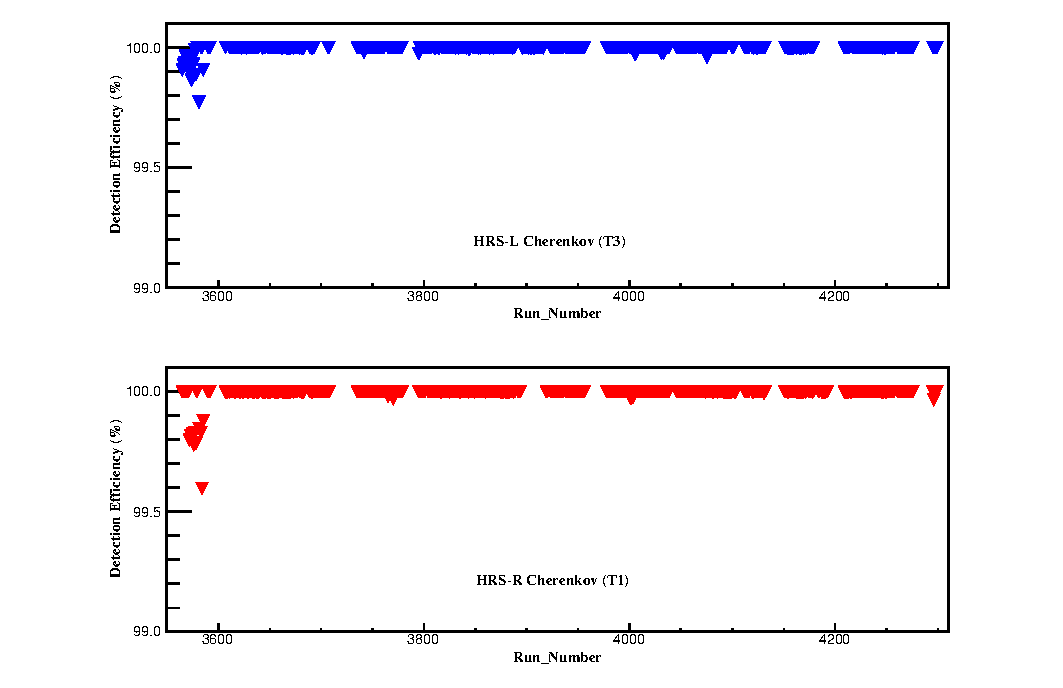
\includegraphics[width=0.7\linewidth]{../figures/cer/Cer_Det_Eff.eps}}
% \caption[Gas Cherenkov Detection Efficiency]{\footnotesize{Gas Cherenkov Detection Efficiency}}
% \label{cer_det_eff}
% \end{figure}

%\begin{figure}[h!]
 \begin{center}
\parbox[t]{0.9\textwidth}{
 \centerline{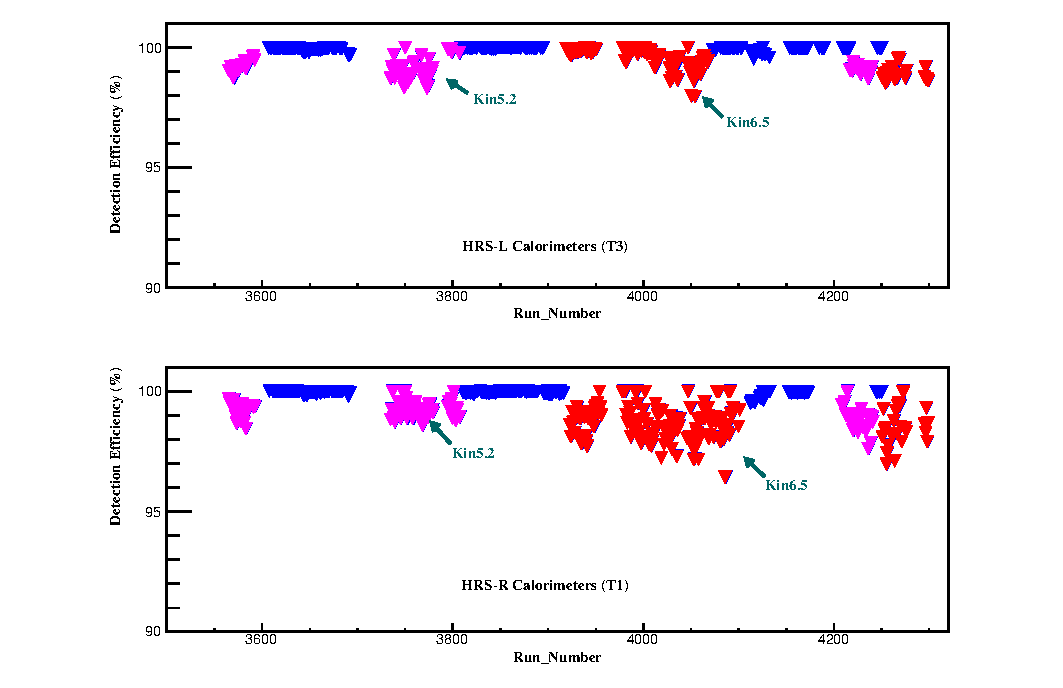
\includegraphics[width=1.\linewidth]{../figures/calo/Calo_Det_Eff1.eps}}
 \captionof{figure}{\footnotesize{Calorimeters: Efficiencies vs Run Number}}
 \label{calo_det_eff}
}
%\end{figure}
\\
%\begin{figure}[h!]
\parbox[t]{0.9\textwidth}{
 \centerline{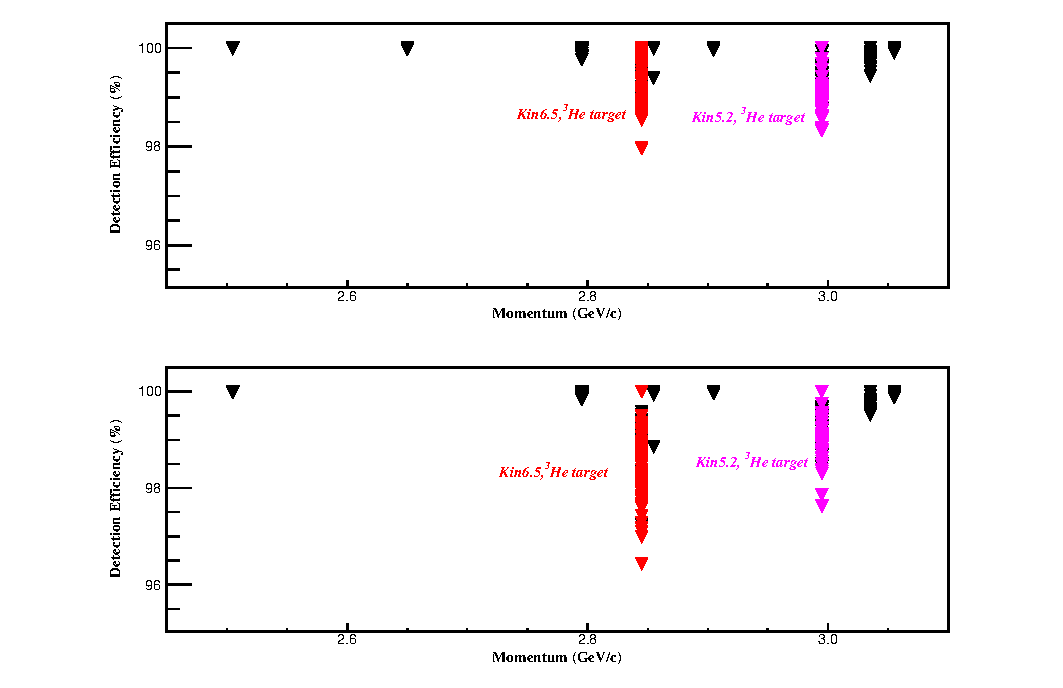
\includegraphics[width=1.\linewidth]{../figures/calo/Calo_Det_Eff_Mom1.eps}}
 \captionof{figure}{\footnotesize{Calorimeters: Efficiency vs Momentum}}
 \label{calo_det_eff_mom}
}
\end{center}
%\end{figure}

%\subsubsection{Calorimeters}
 The detection efficiencies of lead glass calorimeters are expected to be lower than Gas Cherenkov detectors. Calorimeters are composed by piles of lead glass blocks, so the inefficiency of detection is mainly from particles going through gaps in between blocks or hitting the edges or PMT tubes before cascade. Cluster reconstruction when calculating deposited energy in lead glass blocks is another source of inefficiencies, especially when the electron rate is low and many low energy cosmic ray particles mix in.From Fig.\ref{calo_det_eff}, we see that the detection efficiencies of calorimeters on both arm are still high than 99\% for most of runs, but for some runs with low electron rates, mainly for $^{3}He$ target with low beam current (Fig~\ref{calo_det_eff_mom}),the detection efficiencies are slightly lower, due to more cosmic ray contamination. Events from cosmic ray will eventually be removed by applying acceptance cuts and PID cuts, so no correction is necessary for those runs.  


\subsection{Monte Carlo Simulation}

A simulation package, Hall-A Single Arm Monte Carlo (SAMC), which was originally developed by A. Deur \cite{} using FORTRAN and then converted into C++ by Huan Yao \cite{}, is used to study the acceptance effect of HRSs and perform cross section corrections. For each simulation event, its quantities on target plane, $x_{tg},y_{tg}, \theta_{tg}, \phi_{tg}$ and $\delta p_{tg}$, are uniformly generated in a wide phase space. A forward transportation function defines the  geometry of each HRS and transports the target variables to the focal plane if this event can pass through. The calculated focal plane variables are further smeared by introducing VDCs' resolutions, then reconstructed back to the target plane using a back-forward transportation function. Meanwhile, physics quantities, including cross sections, are also calculated for each event. The distribution of reconstructed target plane variables are compared with experiment data to verify the simulation performance. Fig~\ref{samc_tg} compare the distribution of target plane variables between simulation data and experiment data for $^{12}C$ and $^{3}He$, where for simulation data all distributions are weighted by cross sections. Note that for $^{3}He$ target, the well known bump on the vertex distribution can be seen clearly when comparing with simulation data.

\begin{figure}[ht!]
 \begin{center}
 \subfloat[$^{12}C$]{
  \includegraphics[width=0.6\textwidth]{../figures/samc/C12_Com_TG.eps}
 }  
\\
 \subfloat[$^{3}He$]{
  \includegraphics[width=0.6\textwidth]{../figures/samc/He3_Com_TG.eps}
}
 \caption[Comparing MC data and experiment data]{Comparing target plane variables of MC data (blue) and experiment data (red)}
 \label{samc_tg}
\end{center}
\end{figure}


We generate 5 million events which passing through HRSs for each target in each kinematics setting. Since calculating the radiated cross section value for each event takes very long time, we used XEMC cross section package to generate cross section tables for all kinematics settings and look up cross section values from the tables when we further study the simulation data. Detail discussion on XEMC will be discussed in next section. In Eq~\eqref{xs_eq}, $N_{MC}^{gen}$ is equal to total number of events generated in the entire phase space, $\Delta\Omega_{MC}\Delta E'_{MC}$, which is slightly larger than the true coverage of HRSs ($\Delta\delta p=0.12, \Delta\theta_{tg}=0.18, and \Delta\phi_{tg}=0.09$). $N_{MC}^{i}$ is the total number of events in $i$th bin that passing through acceptance cuts of each HRS and being weighted by cross section:
\begin{equation}
  N_{MC}^{i} = \sum_{j\in i} \frac{\sigma_{MC}(E_{0}^{j},E_{p}^{j},\theta^{j})}{\sigma_{MC}(E_{0}^{j},E_{p}^{j},\theta_{0})},
\end{equation}
where $\sum_{j\in i}$ means summarizing all events in $i$th bin,$\sigma_{MC}(E_{0}^{j},E_{p}^{j},\theta^{j})$ is the cross section value for $j$th event, where $E_{0}^{j}$ and $E_{p}^{j}$ are incident and outgoing energies corrected by energy loss, and $\sigma_{MC}(E_{0}^{j},E_{p}^{j},\theta_{0})$ is the cross section value at the central angle $\theta_{0}$. The ratio of $\frac{\sigma_{MC}(E_{0}^{j},E_{p}^{j},\theta^{j})}{\sigma_{MC}(E_{0}^{j},E_{p}^{j},\theta_{0})}$ will automatically do the bin-centering corrections. And $\frac{N_{MC}^{gen}}{N_{MC}^{i} \Delta\Omega_{MC} \Delta E'_{MC}}$ should be able to correct acceptance effects.


\subsection{Cross Section Model}

\subsubsection{XEMC Model} 

 To be added ...

\subsubsection{Cross Section Lookup Tables} 

 In each kinematics settings for each target, we separated a large phase space ($\Delta\delta p=0.14$ and $\Delta\theta=0.20$) into $200 \times 200$ lattices and calculated a radiated cross section value in each lattice point. The results were saved into an ascii text file. Since the bin size is fine enough, we can assume that in each $\delta p$ bin, the values of cross section does not vary too much for difference $\theta$ values, and meanwhile, in each $\theta$ bin, the distribution of cross section as function of $\delta p$ (or $E_{p}$) can be considered to be linear. Base on this assumption, for an event with ($E_{p}, \theta$), we look up the table (Fig~\ref{xs_table}), search for the most close angle value, $\theta^{i}$, as well as two momentum values,$E_{p}^{j}$ and $E_{p}^{j+1}$ (so $E_{p}^{j}<E_{p}<E_{p}^{j+1}$). We can obtain the estimated cross section value for this event using the linear relationship:
\begin{equation}
 \sigma(E_{p},\theta) = \sigma(E_{p}^{j},\theta^{i}) - \frac{E_{p}-E_{p}^{j}}{E_{p}^{j+1}-E_{p}^{j}}(\sigma(E_{p}^{j},\theta^{i})-\sigma(E_{p}^{j+1},\theta^{i}))
\end{equation}
We compared the difference between the table-lookup method and direct calculation, which is less than 0.1\%. 

\subsection{Acceptance and Binning}

\subsubsection{Acceptance Study}
To be added ...

\subsubsection{Binning}

In the code we prepare four variables for binning, $\delta p, \nu, Q^{2}$ and $x_{bj}$, and we can decide which one to use as well as its bin size using a input file outside the code.  We currently only bin on $x_{bj}$ with fix bin size, the value of which for each target depends on kinematics range and statistics, and which could be from 0.01 to 0.1. We used the variable calculated in the physics module in ANALYZER, such as $EKL.x\_bj$ for HRS-L, and defined a binning cut to obtain events inside the $i$th bin:
\begin{equation*}
  |EK.x\_bj - x_{bj}^{i}| <= \Delta_{bin\_size}, \qquad where \quad x_{bi}^{i} = x_{bj}^{min} + (i+1/2)\Delta_{bin\_size}
\end{equation*}

\subsection{Events Selections}
  
There are several cuts applied to select good scattered electron events, for example, for events in HRS-L:

\begin{enumerate}
\item \textbf{$DBB.evtypebits>>3\&1$}, cut on trigger events, $1$ for HRS-R and $3$ for HRS-L\\
\item \textbf{$DBB.edptl[0]==0$}, remove pulse events generated by EDTM modules
\item \textbf{$L.tr.n==1$}, only allow events with one track in VDCs \\
\item \textbf{$|x_{fp}|<=0.75 \&\& |y_{fp}|<=0.55 \&\& |\theta_{fp}|<=0.15 \&\& |\phi_{fp}|<=0.045$}, focal plane acceptance cuts \\
\item \textbf{$|\delta p_{tg}|<=0.03 \&\& |ReactPointZ|<=0.07 \&\& |\theta_{tg}|<=0.03 \&\& |\phi_{tg}|<=0.02$}, target plane acceptance cuts \\
\item \textbf{$L.cer.asum\_c>=50 \&\& epL<=0.5 \&\& L.prl2.e<=100$}, PID cuts for gas Cherekov detectors, and $E/P$ and second layer of calorimeters \\
\item \textbf{$left\_current >= I_{trip}$}, beam trip cuts \\
\item Binning Cuts
\end{enumerate}

The total number of events for a list of runs after the cuts defined above is given by:
\begin{equation}
  N_{EX}^{i} = \sum_{r} \frac{N_{T_{i}}^{r} PS_{T_{i}}^{r}}{LiveTime_{T_{i}}^{r}},
\end{equation}
where $T_{i}$ defines the type of trigger we are interested in, $r$ represents one of runs in the list, $PS_{T_{i}}^{r}$ is the pre-scale factor of this trigger, and $N_{T_{i}}^{r}$ is the total number of events from $T_{i}$ and recorded by DAQ after cutting out beam trip. 

\subsection{Evaluation of Errors}

So far only simple statistics errors are considered. 

\subsection{Cross Section Results}

Here I put some very preliminary cross section results of $^{3}He$ (Fig.\ref{he3_xs}) and $^{12}C$ (Fig.\ref{c12_xs}), and compare them with values calculated from XEMC model:

\begin{figure}[!ht]
 \begin{center}
 \subfloat[$21^{0}$]{
  \includegraphics[width=0.49\textwidth]{../figures/xs/He3_Com_Kin3.2.eps}
 }  
% \hfill
 \subfloat[$23^{0}$]{
  \includegraphics[width=0.49\textwidth]{../figures/xs/He3_Com_Kin4.2.eps}
}
 \hfill
%\\
 \subfloat[$25^{0}$]{
 \includegraphics[width=0.49\textwidth]{../figures/xs/He3_Com_Kin5.2.eps}
}
% \hfill
 \subfloat[$28^{0}$]{
  \includegraphics[width=0.49\textwidth]{../figures/xs/He3_Com_Kin6.5.eps}
}
 \caption[$^{3}He$ Raw Cross Section comparing with XEMC Model]{$^{3}He$ Raw Cross Section comparing with XEMC Model}
 \label{he3_xs}
\end{center}
\end{figure}

\begin{figure}[!ht]
 \begin{center}
 \subfloat[$21^{0}$]{
  \includegraphics[width=0.49\textwidth]{../figures/xs/C12_Com_Kin3.2.eps}
 }  
%\hfill
 \subfloat[$23^{0}$]{
  \includegraphics[width=0.49\textwidth]{../figures/xs/C12_Com_Kin4.2.eps}
}
 \hfill
%\\
 \subfloat[$25^{0}$]{
 \includegraphics[width=0.49\textwidth]{../figures/xs/C12_Com_Kin5.2.eps}
}
%\hfill
 \subfloat[$28^{0}$]{
  \includegraphics[width=0.49\textwidth]{../figures/xs/C12_Com_Kin6.5.eps}
}
 \caption[$^{12}C$ Raw Cross Section comparing with XEMC Model]{$^{12}C$ Raw Cross Section comparing with XEMC Model}
 \label{c12_xs}
\end{center}
\end{figure}

\subsection{Discussion and Conclusion}

\subsubsection{Remaining issues}
 
 From cross sections plots showed above, we see some remain problems that require us to check the cross section extraction method more carefully:
 \begin{enumerate}
\item  Overlap region in the same angle for two settings does not agree well. For $^{3}He$ target, higher momentum settings always have lower cross section values comparing with results from XEMC.     
\item  Cross sections at lower values of $x_{bj}$ are smaller than results from XEMC and at the tail, the values are higher. It seems there are still some acceptance effects that we don't correct completely. I need to check the Monte Carlo data to see whether there are bugs.
\item  Cross section values of $^{12}C$ look better than $^{3}He$. Does it indicate that the effect of the bumps contributes this issues listed above? 
\item   More ...
\end{enumerate}

\subsubsection{How to understand and work with the bumps}

Before we are able to directly calculate the absolute density distributions and hence evaluate the correct total number of scattering centers, we can estimate this distribution from real data with the help of cross section models and simulation data. The vertex distribution along beam direction ($ReactionPoint.Z$) not only includes the information of density distribution, but also contains the acceptance effect and cross section weighting. Since the simulation data with a good cross section model can reproduce close distributions of target variables (Fig.\ref{samc_tg}), and in the simulation we choose uniform target densities, a ratio of normalized histograms filled by real data and simulation data should be able to remove the acceptance effect and physics and the distribution of the ratio histogram should relatively represent the density distribution of the target (Fig.\ref{long_target_dis}).

\begin{figure}[ht]
 \begin{center}
  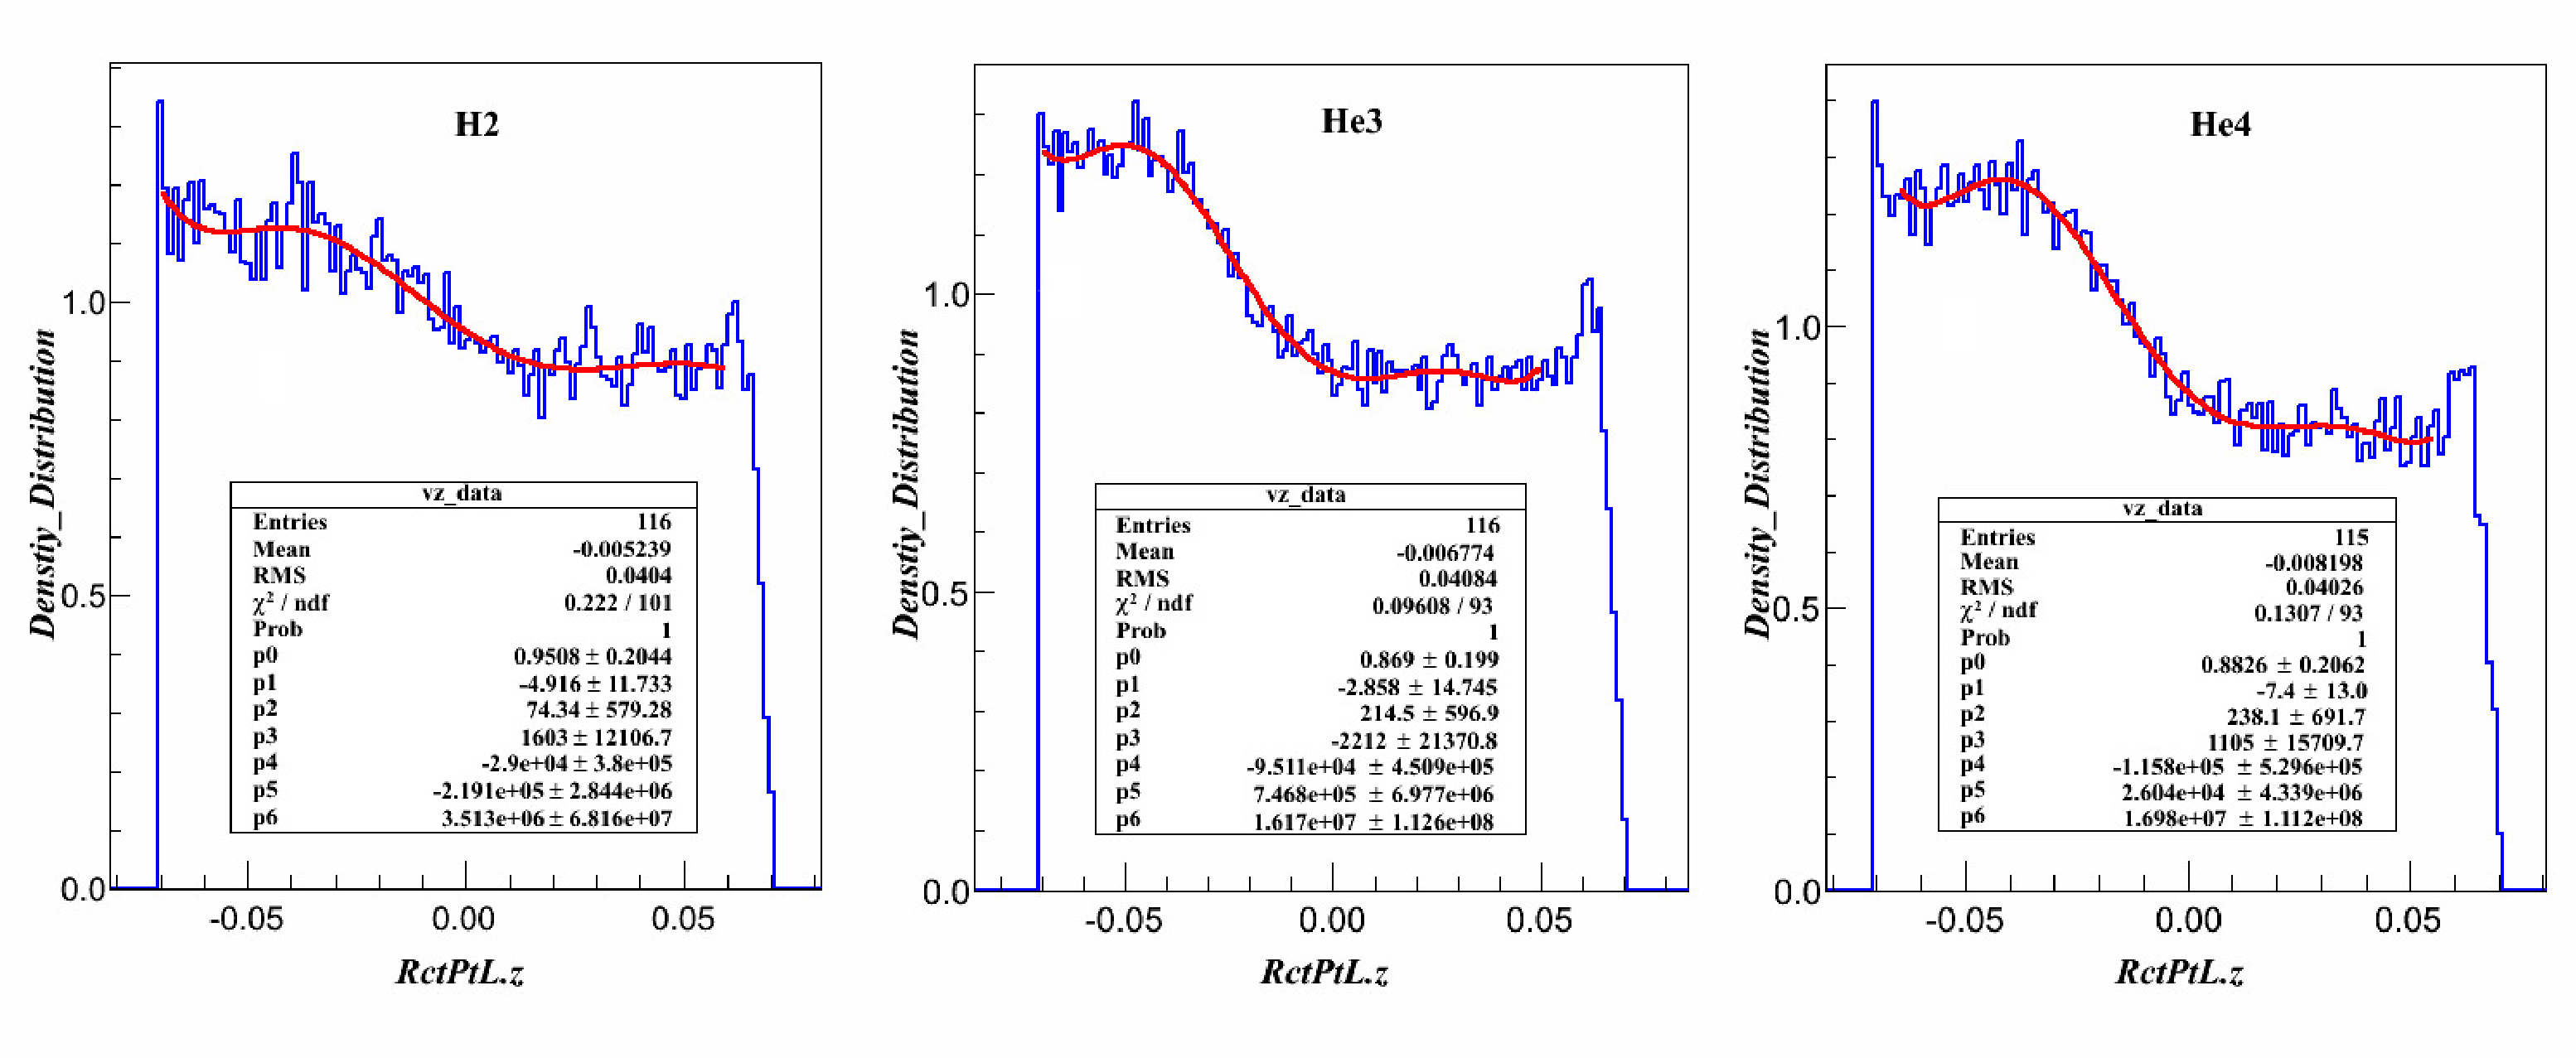
\includegraphics[width=1.0\textwidth]{../figures/target/Target_Bump_Fit.eps}
  \caption[Density distribution of long targets extracted from data]{Density distribution of long targets extracted from data}
  \label{long_target_dis}
 \end{center}
\end{figure}

 From the plots, we concludes that the density of upstream part is roughly 1.25 times larger than the average value while the downstream parts is roughly 0.85 times lower, and the boundary is not that clear. I wrote a step function and introduced the resolution of Vertex Z base on the quantity of optics reconstruction, and compared it with real data, and as you can see from Fig.\ref{long_target_step}, the transaction area does not agree well, which indicates that the target system is more complicate that what we thought. 

\begin{figure}[ht]
 \begin{center}
  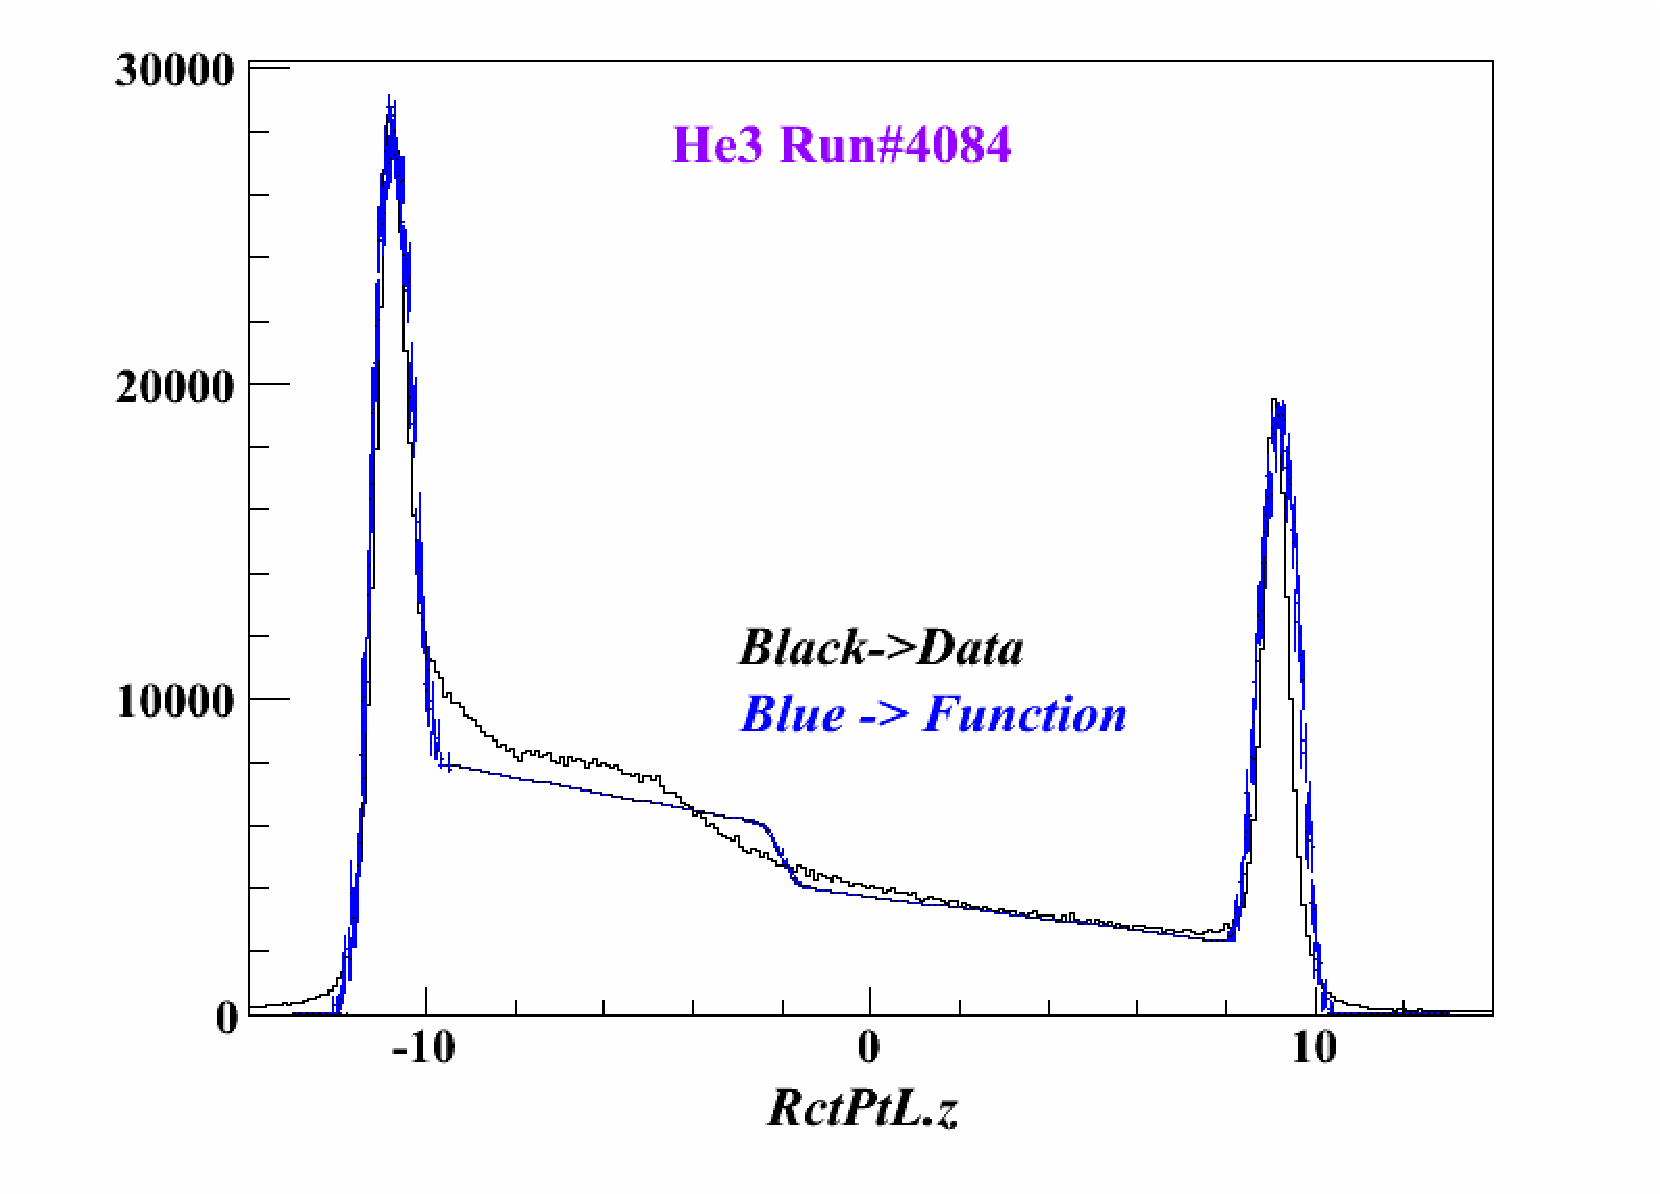
\includegraphics[width=0.6\textwidth]{../figures/target/VZ_Com_True_Resol.eps}
  \caption[Test the density distribution with a step function]{Test the density distribution with a step function}
  \label{long_target_step}
 \end{center}
\end{figure}

The other aspect we need to consider is that whether the non-linearity of long targets affects the distribution of cross section when binning on $x_{bj}$, which depends on scattering angles and hence indirectly depends on target vertex (or equally $Y_{tg}$). We look at the simulation data ($^{3}He$ at Kin3.1) and find out that -- if we make reasonable acceptance cuts and in a fine bin ($\Delta x_{bj} = 0.1$), the distribution of $Y_{tg}$ is flat which indicates that the Yield in one bin does not affected by the bump. 

\begin{figure}[!ht]
 \begin{center}
 \subfloat[w/o acceptance cuts]{
  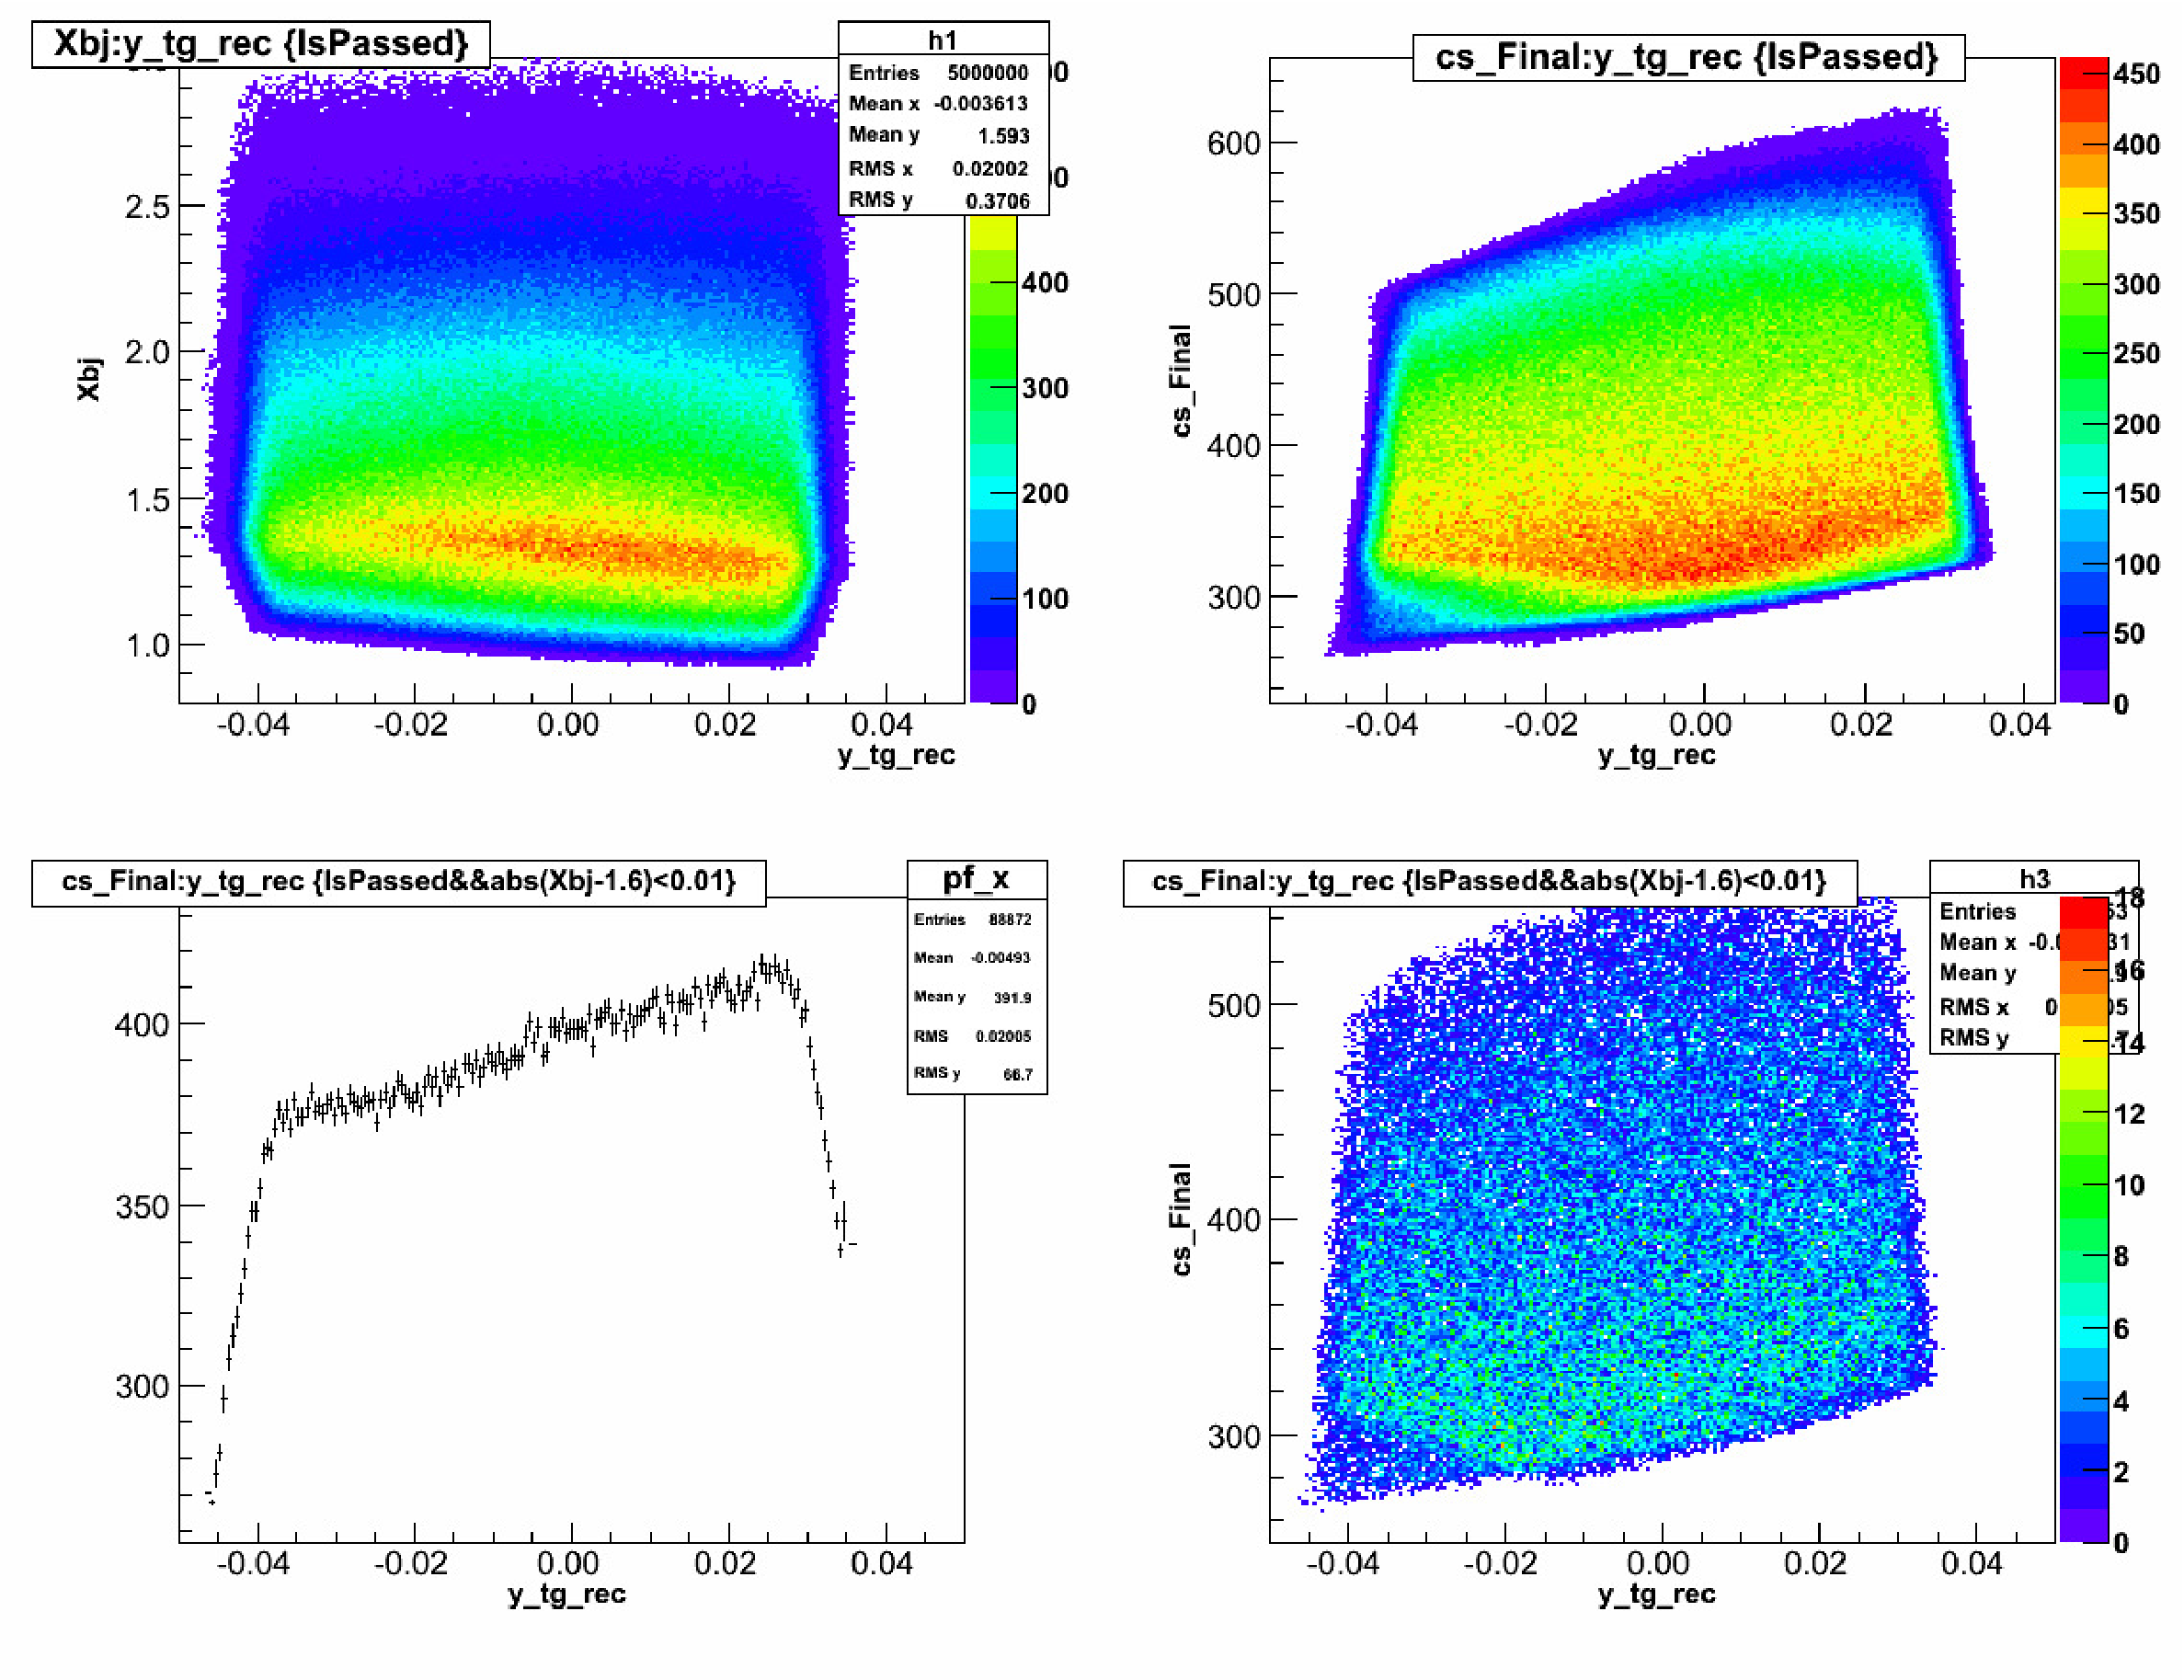
\includegraphics[width=0.8\textwidth]{../figures/target/SAMC_Ytg_Xbj.eps}
}
\\
 \subfloat[w/ acceptance cuts]{
  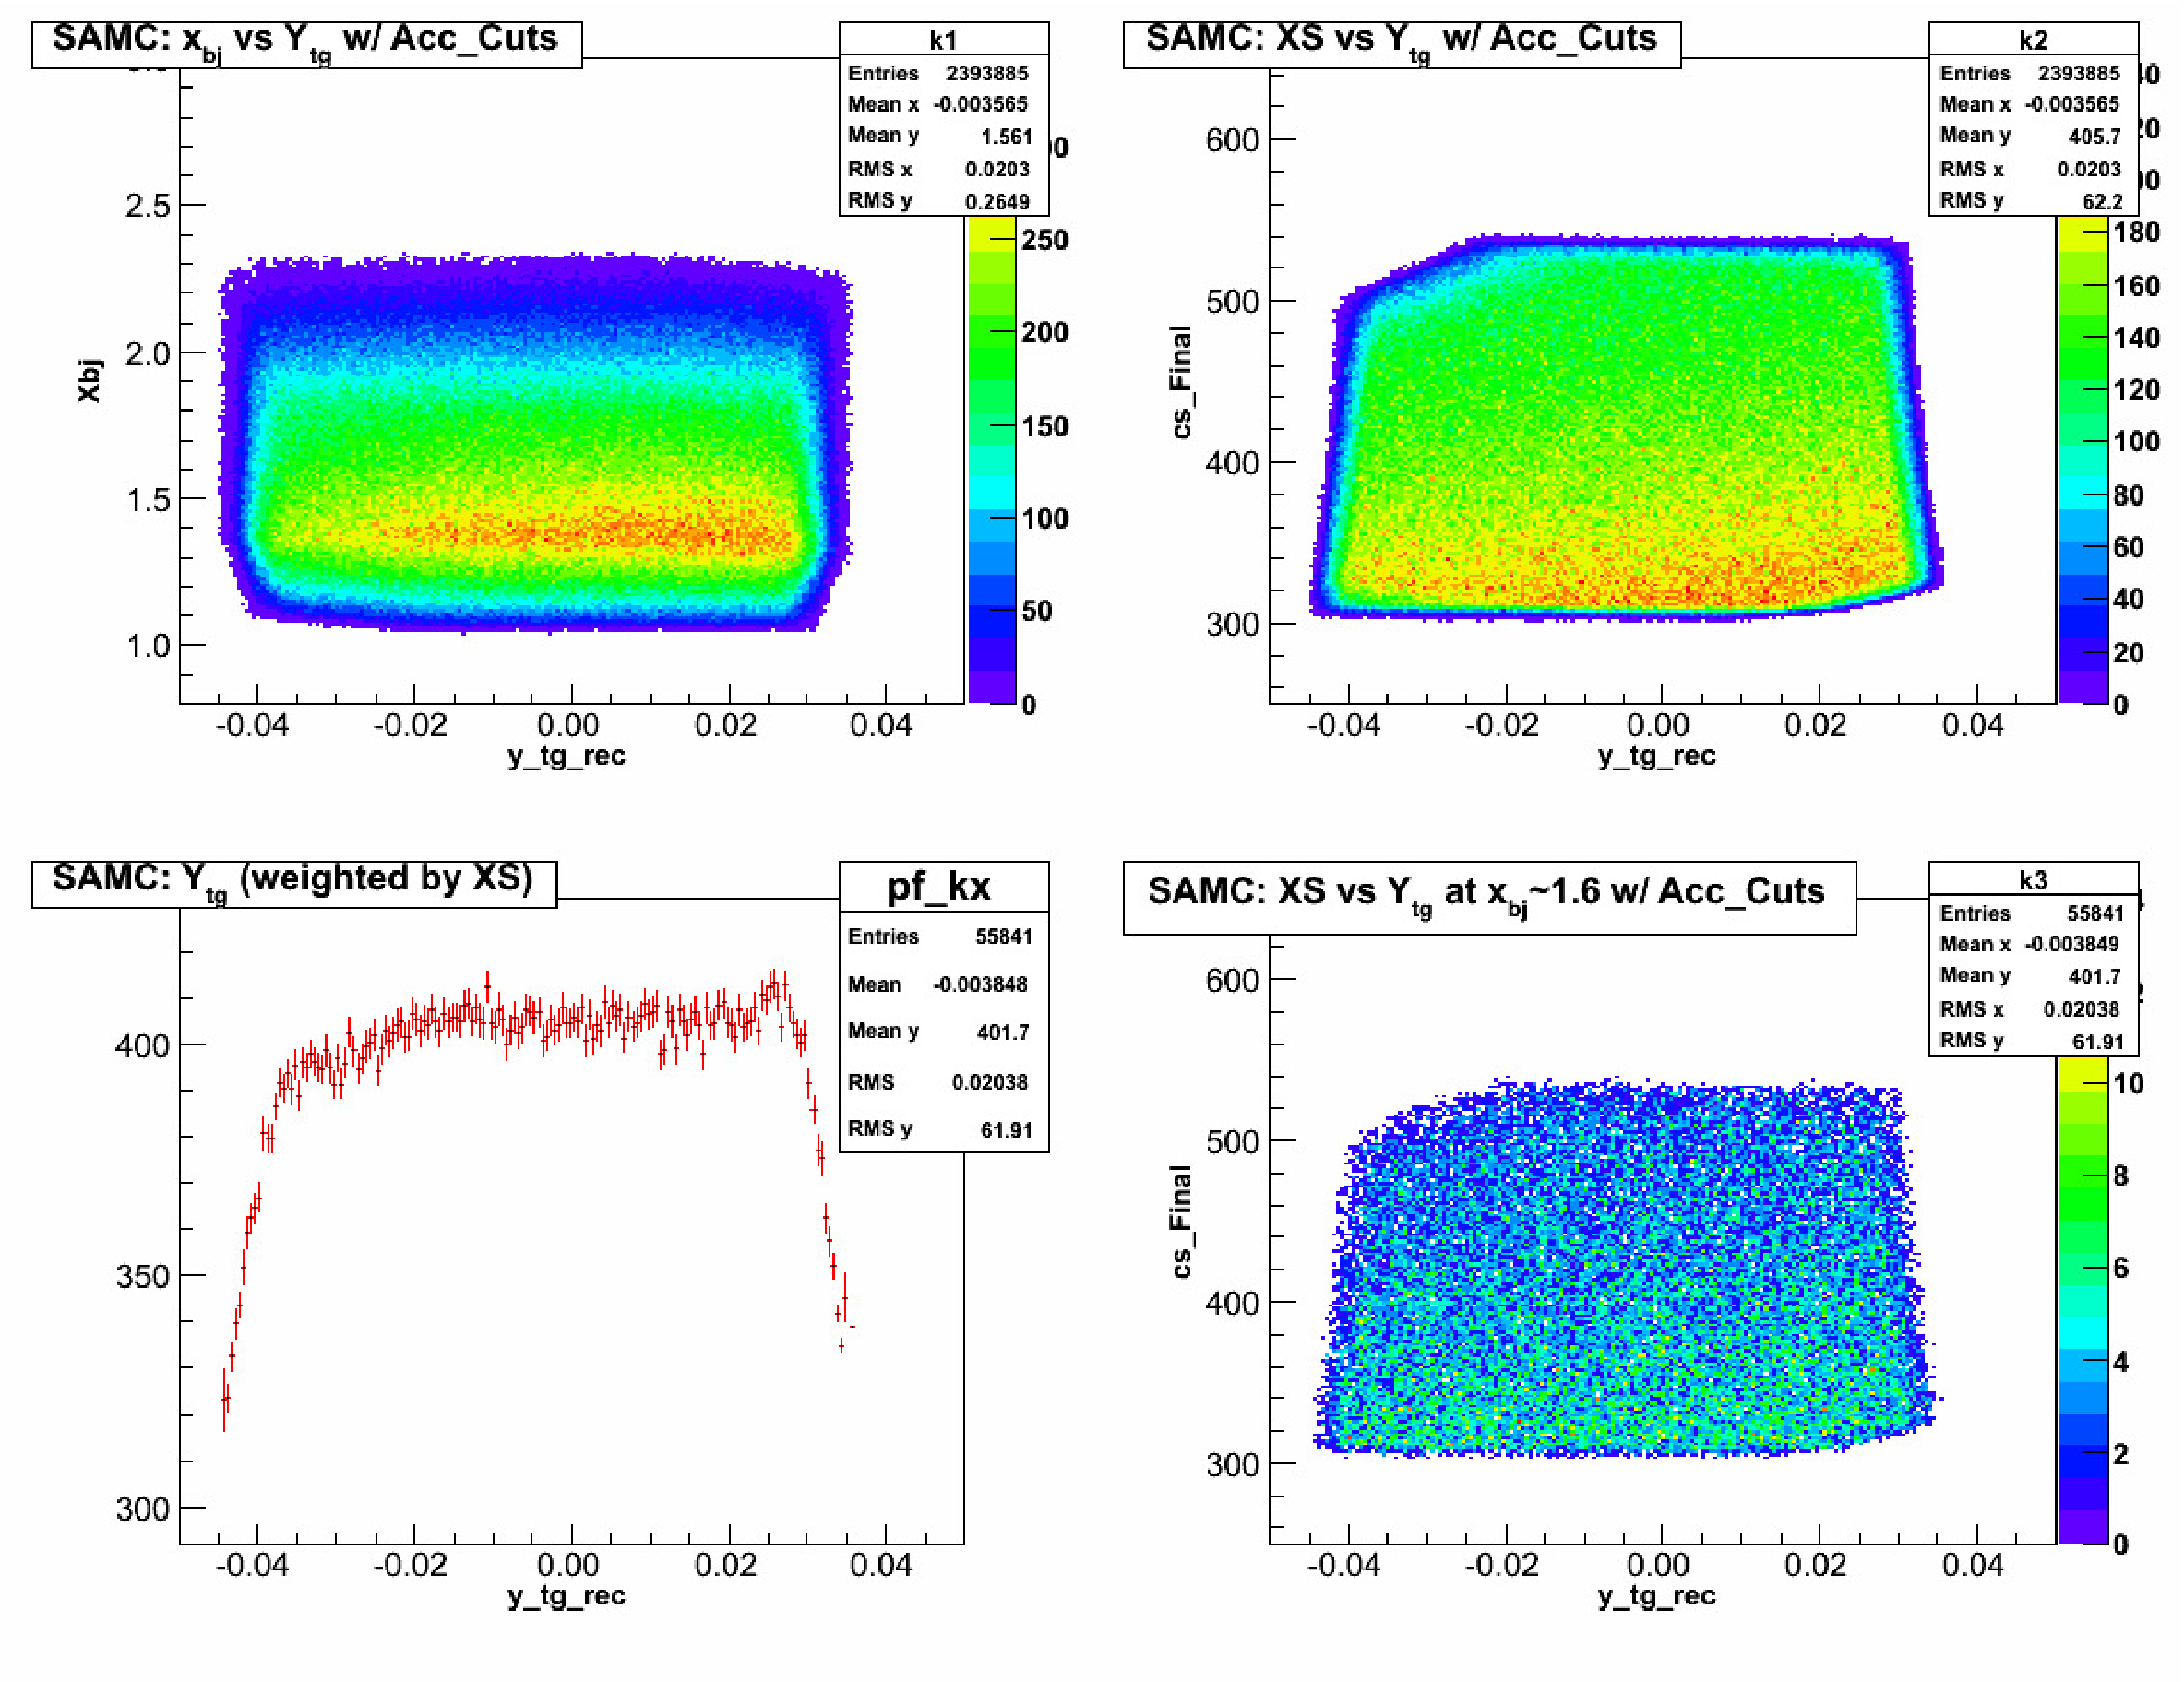
\includegraphics[width=0.8\textwidth]{../figures/target/SAMC_Ytg_Xbj_AccCuts.eps}
}
  \caption[Cross section varying with along targets in simulation]{Cross section varying with along targets in one fine $x_{bj}$ bin using simulation data}
  \label{xs_bump_simu}
 \end{center}
\end{figure}

 Back to experiment data, we plot the correlation of $Y_{tg}$ and $x_{bj}$ (Fig.\ref{xs_bump_data}), where the profile of the 2-D histogram shows the dependence of $Y_{tg}$ on $x_{bj}$. From the plot at middle left, we also see that $x_{bj}$ does not affected by the bump. Base on those two examinations, we can conclude that when calculating raw cross sections, the target issue is not needed to be considered. 

\begin{figure}[!ht]
 \begin{center}
  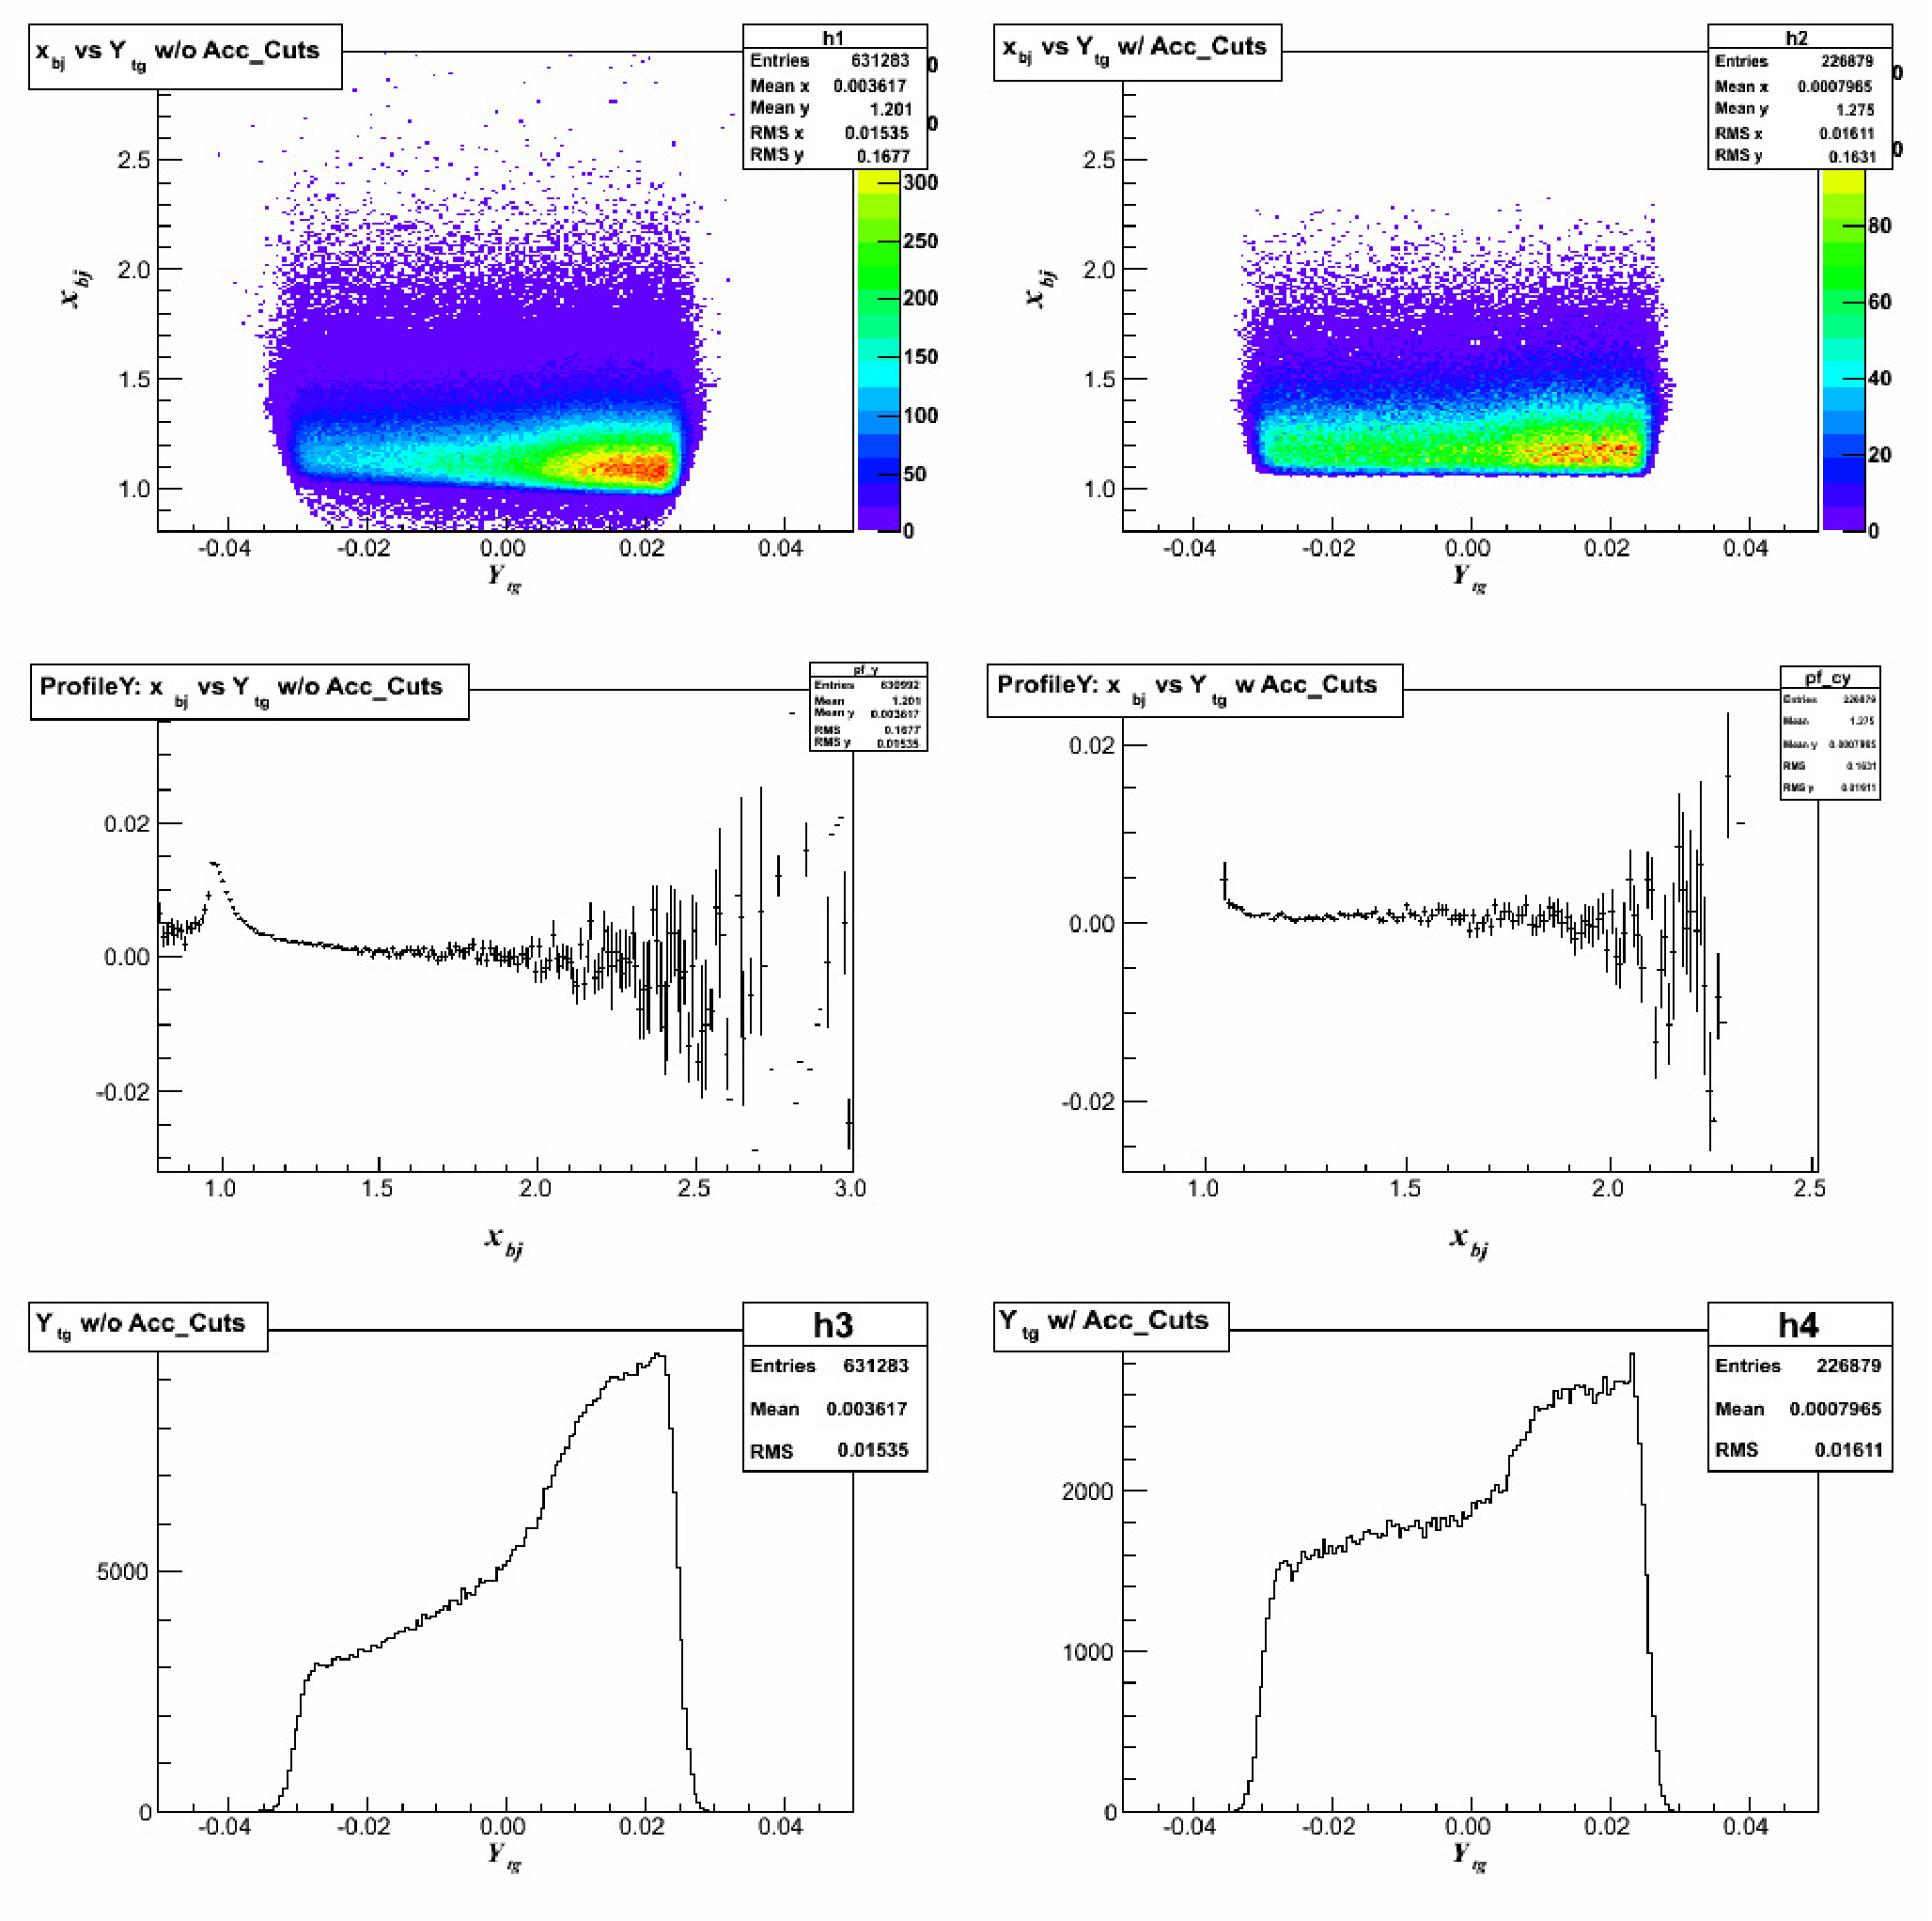
\includegraphics[width=0.6\textwidth]{../figures/target/Data_He3_4085_Ytg_Xbj.eps}
  \caption[Cross section varying with along targets in data]{Cross section varying with along targets in one fine $x_{bj}$ bin using experiment data}
  \label{xs_bump_data}
 \end{center}
\end{figure}

However, special treatments are required when we work on radiated cross sections. Transitionally we assume the reaction points always locates at the center of the target cell, which is a good estimation if the target density is uniform. It will be more complicate if parts of the target have high density and hence cause more reactions than other parts. The study heavily reply on a good radiated cross section model and a Monte Carlo tool. Detail description of how to treat the radiation correction using XEMC model can be found in Elog \#64 or the pdf file attached with this note. Basic idea is that we need to calculate cross sections for one setting ($E0, Ep, and \theta$), but in ten different locations in the target cell. In SAMC, we can modify the generator to generate more statistics on upstream part of long targets, to simulate the truth that more events coming out from the upstream part. Each event with specific $Y_{tg}$ value will look for its most close cross section value from the table. We can adjust the input until the distribution of $Y_{tg}$ for real data and simulation data completely agree with each other. When we calculate $N_{MC}^{i}$ in Eq\eqref{xs_eq}, the effect from long target bumps should be automatically corrected. 

Once we obtain the radiated cross sections from experimental data, we need to know that how the average radiation correction should be with the good understanding of target density at different locations. Work base on this idea is still undergoing.


\end{document}

